% Options for packages loaded elsewhere
\PassOptionsToPackage{unicode}{hyperref}
\PassOptionsToPackage{hyphens}{url}
\PassOptionsToPackage{dvipsnames,svgnames,x11names}{xcolor}
%
\documentclass[
  12pt,
]{book}
\usepackage{amsmath,amssymb}
\usepackage{iftex}
\ifPDFTeX
  \usepackage[T1]{fontenc}
  \usepackage[utf8]{inputenc}
  \usepackage{textcomp} % provide euro and other symbols
\else % if luatex or xetex
  \usepackage{unicode-math} % this also loads fontspec
  \defaultfontfeatures{Scale=MatchLowercase}
  \defaultfontfeatures[\rmfamily]{Ligatures=TeX,Scale=1}
\fi
\usepackage{lmodern}
\ifPDFTeX\else
  % xetex/luatex font selection
  \setmonofont[scale=0.7]{Source Code Pro}
\fi
% Use upquote if available, for straight quotes in verbatim environments
\IfFileExists{upquote.sty}{\usepackage{upquote}}{}
\IfFileExists{microtype.sty}{% use microtype if available
  \usepackage[]{microtype}
  \UseMicrotypeSet[protrusion]{basicmath} % disable protrusion for tt fonts
}{}
\makeatletter
\@ifundefined{KOMAClassName}{% if non-KOMA class
  \IfFileExists{parskip.sty}{%
    \usepackage{parskip}
  }{% else
    \setlength{\parindent}{0pt}
    \setlength{\parskip}{6pt plus 2pt minus 1pt}}
}{% if KOMA class
  \KOMAoptions{parskip=half}}
\makeatother
\usepackage{xcolor}
\usepackage{color}
\usepackage{fancyvrb}
\newcommand{\VerbBar}{|}
\newcommand{\VERB}{\Verb[commandchars=\\\{\}]}
\DefineVerbatimEnvironment{Highlighting}{Verbatim}{commandchars=\\\{\}}
% Add ',fontsize=\small' for more characters per line
\usepackage{framed}
\definecolor{shadecolor}{RGB}{248,248,248}
\newenvironment{Shaded}{\begin{snugshade}}{\end{snugshade}}
\newcommand{\AlertTok}[1]{\textcolor[rgb]{0.94,0.16,0.16}{#1}}
\newcommand{\AnnotationTok}[1]{\textcolor[rgb]{0.56,0.35,0.01}{\textbf{\textit{#1}}}}
\newcommand{\AttributeTok}[1]{\textcolor[rgb]{0.13,0.29,0.53}{#1}}
\newcommand{\BaseNTok}[1]{\textcolor[rgb]{0.00,0.00,0.81}{#1}}
\newcommand{\BuiltInTok}[1]{#1}
\newcommand{\CharTok}[1]{\textcolor[rgb]{0.31,0.60,0.02}{#1}}
\newcommand{\CommentTok}[1]{\textcolor[rgb]{0.56,0.35,0.01}{\textit{#1}}}
\newcommand{\CommentVarTok}[1]{\textcolor[rgb]{0.56,0.35,0.01}{\textbf{\textit{#1}}}}
\newcommand{\ConstantTok}[1]{\textcolor[rgb]{0.56,0.35,0.01}{#1}}
\newcommand{\ControlFlowTok}[1]{\textcolor[rgb]{0.13,0.29,0.53}{\textbf{#1}}}
\newcommand{\DataTypeTok}[1]{\textcolor[rgb]{0.13,0.29,0.53}{#1}}
\newcommand{\DecValTok}[1]{\textcolor[rgb]{0.00,0.00,0.81}{#1}}
\newcommand{\DocumentationTok}[1]{\textcolor[rgb]{0.56,0.35,0.01}{\textbf{\textit{#1}}}}
\newcommand{\ErrorTok}[1]{\textcolor[rgb]{0.64,0.00,0.00}{\textbf{#1}}}
\newcommand{\ExtensionTok}[1]{#1}
\newcommand{\FloatTok}[1]{\textcolor[rgb]{0.00,0.00,0.81}{#1}}
\newcommand{\FunctionTok}[1]{\textcolor[rgb]{0.13,0.29,0.53}{\textbf{#1}}}
\newcommand{\ImportTok}[1]{#1}
\newcommand{\InformationTok}[1]{\textcolor[rgb]{0.56,0.35,0.01}{\textbf{\textit{#1}}}}
\newcommand{\KeywordTok}[1]{\textcolor[rgb]{0.13,0.29,0.53}{\textbf{#1}}}
\newcommand{\NormalTok}[1]{#1}
\newcommand{\OperatorTok}[1]{\textcolor[rgb]{0.81,0.36,0.00}{\textbf{#1}}}
\newcommand{\OtherTok}[1]{\textcolor[rgb]{0.56,0.35,0.01}{#1}}
\newcommand{\PreprocessorTok}[1]{\textcolor[rgb]{0.56,0.35,0.01}{\textit{#1}}}
\newcommand{\RegionMarkerTok}[1]{#1}
\newcommand{\SpecialCharTok}[1]{\textcolor[rgb]{0.81,0.36,0.00}{\textbf{#1}}}
\newcommand{\SpecialStringTok}[1]{\textcolor[rgb]{0.31,0.60,0.02}{#1}}
\newcommand{\StringTok}[1]{\textcolor[rgb]{0.31,0.60,0.02}{#1}}
\newcommand{\VariableTok}[1]{\textcolor[rgb]{0.00,0.00,0.00}{#1}}
\newcommand{\VerbatimStringTok}[1]{\textcolor[rgb]{0.31,0.60,0.02}{#1}}
\newcommand{\WarningTok}[1]{\textcolor[rgb]{0.56,0.35,0.01}{\textbf{\textit{#1}}}}
\usepackage{longtable,booktabs,array}
\usepackage{calc} % for calculating minipage widths
% Correct order of tables after \paragraph or \subparagraph
\usepackage{etoolbox}
\makeatletter
\patchcmd\longtable{\par}{\if@noskipsec\mbox{}\fi\par}{}{}
\makeatother
% Allow footnotes in longtable head/foot
\IfFileExists{footnotehyper.sty}{\usepackage{footnotehyper}}{\usepackage{footnote}}
\makesavenoteenv{longtable}
\usepackage{graphicx}
\makeatletter
\def\maxwidth{\ifdim\Gin@nat@width>\linewidth\linewidth\else\Gin@nat@width\fi}
\def\maxheight{\ifdim\Gin@nat@height>\textheight\textheight\else\Gin@nat@height\fi}
\makeatother
% Scale images if necessary, so that they will not overflow the page
% margins by default, and it is still possible to overwrite the defaults
% using explicit options in \includegraphics[width, height, ...]{}
\setkeys{Gin}{width=\maxwidth,height=\maxheight,keepaspectratio}
% Set default figure placement to htbp
\makeatletter
\def\fps@figure{htbp}
\makeatother
\setlength{\emergencystretch}{3em} % prevent overfull lines
\providecommand{\tightlist}{%
  \setlength{\itemsep}{0pt}\setlength{\parskip}{0pt}}
\setcounter{secnumdepth}{5}
\usepackage{booktabs}
\ifLuaTeX
  \usepackage{selnolig}  % disable illegal ligatures
\fi
\usepackage[]{natbib}
\bibliographystyle{apalike}
\usepackage{bookmark}
\IfFileExists{xurl.sty}{\usepackage{xurl}}{} % add URL line breaks if available
\urlstyle{same}
\hypersetup{
  pdftitle={scMINER: a mutual information-based framework for identifying hidden drivers from single-cell omics data},
  pdfauthor={John Doe},
  colorlinks=true,
  linkcolor={Maroon},
  filecolor={Maroon},
  citecolor={Blue},
  urlcolor={Blue},
  pdfcreator={LaTeX via pandoc}}

\title{scMINER: a mutual information-based framework for identifying hidden drivers from single-cell omics data}
\author{John Doe}
\date{2024-08-04}

\begin{document}
\maketitle

{
\hypersetup{linkcolor=}
\setcounter{tocdepth}{1}
\tableofcontents
}
\listoffigures
\listoftables
Welcome to scMINER documentation!

\textbf{scMINER} (\textbf{s}ingle-\textbf{c}ell \textbf{M}utual \textbf{I}nformation-based \textbf{N}etwork \textbf{E}ngineering \textbf{R}anger) is a computational framework designed for \textbf{end-to-end} analysis of single cell RNA-seq data. Using \href{https://en.wikipedia.org/wiki/Mutual_information}{\textbf{mutual information}} to measure cell-cell similarities and gene-gene correlations, scMINER is widely applicable and highly accurate in unsupervised clustering and gene activity inference of scRNA-seq data.

In this documentation, we will walk you through every analysis that scMINER can do and introduce you more about the concepts related to scMINER framework.

\chapter{Introduction}\label{introduction}

This chapter will introduce some principal concepts and unique features of scMINER.

\section{A few concepts}\label{a-few-concepts}

There are a few concepts that may help you understand scMINER better.

\subsection*{SparseEset}\label{sparseeset}
\addcontentsline{toc}{subsection}{SparseEset}

The \textbf{\texttt{SparseExpressionSet}} (or \textbf{\texttt{SparseEset}} for short) is a new class created by scMINER to handle the sparsity in scRNA-seq data. It is derived from \href{https://www.bioconductor.org/packages/release/bioc/vignettes/Biobase/inst/doc/ExpressionSetIntroduction.pdf}{ExpressionSet}, and enables to compress, store and access efficiently and conveniently.

The SparseEset object is the \textbf{center} of scRNA-seq data analysis by scMINER.

\subsection*{Mutual Information}\label{mutual-information}
\addcontentsline{toc}{subsection}{Mutual Information}

\href{https://en.wikipedia.org/wiki/Mutual_information}{Mutual information} is a measure of the mutual dependence between two random variables. It quantifies the amount of information obtained about one variable through the other variable. In other words, it measures how much knowing the value of one variable reduces uncertainty about the value of the other variable. It's widely used in probability theory and information theory.

Compared with the linear correlation that used by most existing tools for scRNA-seq data clustering, mutual information provides a \textbf{more general measure} of dependence that can capture \textbf{\emph{both linear and non-linear relationships}}, and hence may increases the accuracy and sensitivity of scRNA-seq data clustering.

\begin{longtable}[]{@{}
  >{\raggedright\arraybackslash}p{(\columnwidth - 4\tabcolsep) * \real{0.3333}}
  >{\raggedright\arraybackslash}p{(\columnwidth - 4\tabcolsep) * \real{0.3333}}
  >{\raggedright\arraybackslash}p{(\columnwidth - 4\tabcolsep) * \real{0.3333}}@{}}
\caption{\textbf{Comparison of Linear Correlation and Mutual Information (powered by ChatGPT)}}\tabularnewline
\toprule\noalign{}
\begin{minipage}[b]{\linewidth}\raggedright
\end{minipage} & \begin{minipage}[b]{\linewidth}\raggedright
Linear Correlation
\end{minipage} & \begin{minipage}[b]{\linewidth}\raggedright
Mutual Information
\end{minipage} \\
\midrule\noalign{}
\endfirsthead
\toprule\noalign{}
\begin{minipage}[b]{\linewidth}\raggedright
\end{minipage} & \begin{minipage}[b]{\linewidth}\raggedright
Linear Correlation
\end{minipage} & \begin{minipage}[b]{\linewidth}\raggedright
Mutual Information
\end{minipage} \\
\midrule\noalign{}
\endhead
\bottomrule\noalign{}
\endlastfoot
Definition & Measures linear relationship & Measures mutual dependence (both linear and non-linear) \\
Range & -1 to 1 & 0 to Inf \\
Sensitivity to outliers & Sensitive & Less sensitive \\
Captures Non-linear Relationships & No & Yes \\
Common Applications & Regression, finance, science & Feature selection, clustering, network inference \\
\end{longtable}

\subsection*{Gene Activity}\label{gene-activity}
\addcontentsline{toc}{subsection}{Gene Activity}

The gene activity estimation is one of the most important features of scMINER. \textbf{\emph{Mathematically}}, the activity of one gene is a type of mean of the expressions of its targets. And \textbf{\emph{biologically}}, the activity can be interpreted as a measure that describes how actively the driver functions, like the enzymes in digesting their subtracts, kinase in activating their downstream genes. Given the gene expression profiles and networks, scMINER can estimate the activities of some predefined drivers, including not only transcription factors (TFs) but also signaling genes (SIGs).

\section{Why use scMINER}\label{why-use-scminer}

(more details to be added)

scMINER includes the following key functions:

\begin{itemize}
\item
  \textbf{Mutual information-based clustering}: scMINER measures the cell-cell similarities with \textbf{full feature-derived mutual information}. It can catch both linear and non-linear correlations and performs better in cell clustering, especially for those of close states.
\item
  \textbf{Gene activity estimation}: scMINER rewires the cell-type specific gene networks solely from the scRNA-seq data, and then estimates the gene activities of not only \textbf{transcription factors (TFs)} but also \textbf{signaling genes (SIGs)}. The gene activity-based analysis can expose the \textbf{main regulators of various biological activities}, like cellular linage differentiation and tissue specificity.
\item
  \textbf{SparseEset-centered full-feature tool}: scMINER provides a wide range of functions for \textbf{data intake}, \textbf{quality control and filtration}, \textbf{MI-based clustering}, \textbf{network inference}, \textbf{gene activity estimation}, \textbf{cell type annotation}, \textbf{differential expression/activity analysis}, and \textbf{data visualization and sharing}. Most of these functions are developed in an object-oriented manner for the \textbf{SparseEset object}.
\end{itemize}

\section{Citation}\label{citation}

Please consider citing \href{https://www.biorxiv.org/content/10.1101/2023.01.26.523391v1}{this paper} if you find scMINER useful in your research.

\section{Support}\label{support}

We welcome your feedback! The scMINER software is developed and maintained by the \href{https://www.stjude.org/research/labs/yu-lab.html}{Yu Lab @ St.~Jude Children's Research Hospital} and is released under the Apache License (Version 2.0). Feel free to open an \href{https://github.com/jyyulab/scMINER/issues}{issue}, or send us an \href{mailto:jiyang.yu@stjude.org}{email} if you encounter a bug, need our help or just want to make a comment/suggestion.

\chapter{Get started}\label{get-started}

This chapter will walk you through how to install scMINER, create a project space for your study and prepare the demo data used in this tutorial.

\section{Installation}\label{installation}

scMINER framework is mainly developed with R for its advantages in statistical analysis and data visualization. It also includes two components, \href{https://github.com/jyyulab/MICA}{MICA} and \href{https://github.com/jyyulab/SJARACNe}{SJARACNe}, that are developed with Python to take its strengths in calculation speed and memory consumption, since mutual information estimation of large-scale scRNA-seq data is usually compute-intensive.

Please install all three components for the full access to scMINER framework.

\subsection*{Install scMINER R package}\label{install-scminer-r-package}
\addcontentsline{toc}{subsection}{Install scMINER R package}

The scMINER R package requires R 4.2.3 or newer, and can be installed from \href{https://github.com/}{GitHub} with:

\begin{Shaded}
\begin{Highlighting}[]
\CommentTok{\# install.packages("devtools")}
\NormalTok{devtools}\SpecialCharTok{::}\FunctionTok{install\_github}\NormalTok{(}\StringTok{"https://github.com/jyyulab/scMINER.git@dev{-}qpan"}\NormalTok{)}
\end{Highlighting}
\end{Shaded}

\subsection*{Install MICA and SJARACNe}\label{install-mica-and-sjaracne}
\addcontentsline{toc}{subsection}{Install MICA and SJARACNe}

The recommended method to install MICA and SJARACNe is to use \href{https://conda.io/projects/conda/en/latest/}{conda} dependency manager:

\begin{Shaded}
\begin{Highlighting}[]
\CommentTok{\#\# setup conda env}
\ExtensionTok{conda}\NormalTok{ create }\AttributeTok{{-}n}\NormalTok{ scminer python=3.9.2                }\CommentTok{\# Create a python virtual environment}
\BuiltInTok{source}\NormalTok{ activate scminer                             }\CommentTok{\# Activate the virtual environment}

\CommentTok{\#\# install MICA}
\FunctionTok{git}\NormalTok{ clone https://github.com/jyyulab/MICA           }\CommentTok{\# Clone the MICA repo}
\BuiltInTok{cd}\NormalTok{ MICA                                             }\CommentTok{\# Switch to the MICA root directory}
\ExtensionTok{pip}\NormalTok{ install .                                       }\CommentTok{\# Install MICA and its dependencies}
\ExtensionTok{mica} \AttributeTok{{-}h}                                             \CommentTok{\# Check if MICA works}

\CommentTok{\#\# install SJARACNE}
\BuiltInTok{cd}\NormalTok{ ..                                               }\CommentTok{\# Switch to conda env folder}
\FunctionTok{git}\NormalTok{ clone https://github.com/jyyulab/SJARACNe.git   }\CommentTok{\# Clone the SJARACNe repo}
\BuiltInTok{cd}\NormalTok{ SJARACNe                                         }\CommentTok{\# Switch to the MICA root directory}
\ExtensionTok{python}\NormalTok{ setup.py build                               }\CommentTok{\# Build SJARACNe binary}
\ExtensionTok{python}\NormalTok{ setup.py install                             }\CommentTok{\# Build SJARACNe binary}
\ExtensionTok{sjaracne} \AttributeTok{{-}h}                                         \CommentTok{\# Check if SJARACNe works}
\end{Highlighting}
\end{Shaded}

\section{Demo data}\label{demo-data}

In this tutorial, we will use a \textbf{\emph{ground truth}} dataset called \textbf{PBMC14k} for demonstration purposes. It was generated from a Peripheral Blood Mononuclear Cells (PBMCs) dataset containing 10 known cell types, with 2,000 cells per type {[}\href{./data-reference.md\#\%5BZheng\%20et\%20al.,\%202017\%5D}{Zheng et al., 2017}{]}:

\begin{enumerate}
\def\labelenumi{\arabic{enumi}.}
\tightlist
\item
  We first rectified the gene symbol issues of the original dataset, including the dash-dot conversion (e.g.~``RP11-34P13.7'' changed to ``RP11.34P13.7'') and ``X'' added to those started with numbers (e.g.~``7SK'' changed to ``X7SK''), by referring to the gene annotation file (GRCh37.82) used in the original study.
\item
  Then we removed 3 cell populations, CD34+ cells, CD4+ helper T cells, and total CD8+ cytotoxic cells, from the dataset because of either low sorting purity or a significant overlap with other immune cells based on the sorting strategy, and created a new dataset with seven known cell types and 14k cells in total.
\end{enumerate}

The original dataset is freely available under this accession number \href{https://www.ncbi.nlm.nih.gov/sra?term=SRP073767}{SRP073767} and \href{https://zenodo.org/record/3357167\#.YhQNF2RKj6V}{Zenodo}.

\textbf{How was the PBMC14K dataset generated from the original dataset?}

\begin{Shaded}
\begin{Highlighting}[]
\DocumentationTok{\#\# Step 1: rectify the invalid gene symbols}
\CommentTok{\# "Filtered\_DownSampled\_SortedPBMC\_data.csv" is the raw count matrix directly downloaded from Zenodo}
\NormalTok{counts }\OtherTok{\textless{}{-}} \FunctionTok{read.csv}\NormalTok{(}\StringTok{"Filtered\_DownSampled\_SortedPBMC\_data.csv"}\NormalTok{, }\AttributeTok{row.names =} \DecValTok{1}\NormalTok{) }
\NormalTok{d }\OtherTok{\textless{}{-}} \FunctionTok{t}\NormalTok{(counts); }\FunctionTok{dim}\NormalTok{(d) }\CommentTok{\# it includes 21592 genes and 20000 cells}

\CommentTok{\# "genesymbol\_from\_GTF\_GRCh37.txt" contains the official gene ids and symbols extracted from GTF file downloaded from}
\NormalTok{officialGene }\OtherTok{\textless{}{-}} \FunctionTok{read.table}\NormalTok{(}\StringTok{"genesymbol\_from\_GTF\_GRCh37.txt"}\NormalTok{, }\AttributeTok{header =}\NormalTok{ T, }\AttributeTok{sep =} \StringTok{"}\SpecialCharTok{\textbackslash{}t}\StringTok{"}\NormalTok{, }\AttributeTok{quote =} \StringTok{""}\NormalTok{, }\AttributeTok{stringsAsFactors =}\NormalTok{ F); }\FunctionTok{head}\NormalTok{(officialGene)  https}\SpecialCharTok{:}\ErrorTok{//}\NormalTok{ftp.ensembl.org}\SpecialCharTok{/}\NormalTok{pub}\SpecialCharTok{/}\NormalTok{grch37}\SpecialCharTok{/}\NormalTok{current}\SpecialCharTok{/}\NormalTok{gtf}\SpecialCharTok{/}\NormalTok{homo\_sapiens}\SpecialCharTok{/}
\NormalTok{officialGene}\SpecialCharTok{$}\NormalTok{dotted\_symbol }\OtherTok{\textless{}{-}} \FunctionTok{gsub}\NormalTok{(}\StringTok{"{-}"}\NormalTok{, }\StringTok{"}\SpecialCharTok{\textbackslash{}\textbackslash{}}\StringTok{."}\NormalTok{, officialGene}\SpecialCharTok{$}\NormalTok{gene\_name); officialGene}\SpecialCharTok{$}\NormalTok{dotted\_symbol }\OtherTok{\textless{}{-}} \FunctionTok{make.unique}\NormalTok{(officialGene}\SpecialCharTok{$}\NormalTok{dotted\_symbol)}
\FunctionTok{table}\NormalTok{(}\FunctionTok{row.names}\NormalTok{(d) }\SpecialCharTok{\%in\%}\NormalTok{ officialGene}\SpecialCharTok{$}\NormalTok{dotted\_symbol); }\FunctionTok{row.names}\NormalTok{(d)[}\SpecialCharTok{!} \FunctionTok{row.names}\NormalTok{(d) }\SpecialCharTok{\%in\%}\NormalTok{ officialGene}\SpecialCharTok{$}\NormalTok{dotted\_symbol] }\CommentTok{\# two genes are not in: X7SK.1 and X7SK.2}
\FunctionTok{row.names}\NormalTok{(d) }\OtherTok{\textless{}{-}} \FunctionTok{gsub}\NormalTok{(}\StringTok{"X7SK.1"}\NormalTok{, }\StringTok{"7SK"}\NormalTok{, }\FunctionTok{row.names}\NormalTok{(d)); }\FunctionTok{row.names}\NormalTok{(d) }\OtherTok{\textless{}{-}} \FunctionTok{gsub}\NormalTok{(}\StringTok{"X7SK.2"}\NormalTok{, }\StringTok{"7SK.1"}\NormalTok{, }\FunctionTok{row.names}\NormalTok{(d))}
\FunctionTok{table}\NormalTok{(}\FunctionTok{row.names}\NormalTok{(d) }\SpecialCharTok{\%in\%}\NormalTok{ officialGene}\SpecialCharTok{$}\NormalTok{dotted\_symbol) }\CommentTok{\# all true}
\FunctionTok{row.names}\NormalTok{(officialGene) }\OtherTok{\textless{}{-}}\NormalTok{ officialGene}\SpecialCharTok{$}\NormalTok{dotted\_symbol}
\NormalTok{officialGene }\OtherTok{\textless{}{-}}\NormalTok{ officialGene[}\FunctionTok{row.names}\NormalTok{(d),]}
\FunctionTok{row.names}\NormalTok{(d) }\OtherTok{\textless{}{-}} \FunctionTok{make.unique}\NormalTok{(officialGene}\SpecialCharTok{$}\NormalTok{gene\_name)}

\CommentTok{\# "Labels.csv" contains the true labels of cell types and was directly downloaded from Zenodo}
\NormalTok{celltype }\OtherTok{\textless{}{-}} \FunctionTok{read.csv}\NormalTok{(}\StringTok{"Labels.csv"}\NormalTok{); }\FunctionTok{head}\NormalTok{(celltype); }
\FunctionTok{table}\NormalTok{(celltype}\SpecialCharTok{$}\NormalTok{x) }\CommentTok{\# 2000 cells for each of 10 cell types: CD14+ Monocyte, CD19+ B, CD34+, CD4+ T Helper2, CD4+/CD25 T Reg, CD4+/CD45RA+/CD25{-} Naive T, CD4+/CD45RO+ Memory, CD56+ NK, CD8+ Cytotoxic T, CD8+/CD45RA+ Naive Cytotoxic}
\NormalTok{df }\OtherTok{\textless{}{-}} \FunctionTok{data.frame}\NormalTok{(}\AttributeTok{cell\_barcode =} \FunctionTok{colnames}\NormalTok{(d), }\AttributeTok{trueLabel\_full =}\NormalTok{ celltype}\SpecialCharTok{$}\NormalTok{x); }\FunctionTok{dim}\NormalTok{(df)}
\NormalTok{truelabel\_map }\OtherTok{\textless{}{-}} \FunctionTok{c}\NormalTok{(}\StringTok{\textasciigrave{}}\AttributeTok{CD14+ Monocyte}\StringTok{\textasciigrave{}}\OtherTok{=}\StringTok{"Monocyte"}\NormalTok{, }\StringTok{\textasciigrave{}}\AttributeTok{CD19+ B}\StringTok{\textasciigrave{}}\OtherTok{=}\StringTok{"B"}\NormalTok{, }\StringTok{\textasciigrave{}}\AttributeTok{CD34+}\StringTok{\textasciigrave{}}\OtherTok{=}\StringTok{"CD34pos"}\NormalTok{, }\StringTok{\textasciigrave{}}\AttributeTok{CD4+ T Helper2}\StringTok{\textasciigrave{}}\OtherTok{=}\StringTok{"CD4Th2"}\NormalTok{, }\StringTok{\textasciigrave{}}\AttributeTok{CD4+/CD25 T Reg}\StringTok{\textasciigrave{}}\OtherTok{=}\StringTok{"CD4Treg"}\NormalTok{,}
                  \StringTok{\textasciigrave{}}\AttributeTok{CD4+/CD45RA+/CD25{-} Naive T}\StringTok{\textasciigrave{}}\OtherTok{=}\StringTok{"CD4TN"}\NormalTok{, }\StringTok{\textasciigrave{}}\AttributeTok{CD4+/CD45RO+ Memory}\StringTok{\textasciigrave{}}\OtherTok{=}\StringTok{"CD4TCM"}\NormalTok{, }\StringTok{\textasciigrave{}}\AttributeTok{CD56+ NK}\StringTok{\textasciigrave{}}\OtherTok{=}\StringTok{"NK"}\NormalTok{, }\StringTok{\textasciigrave{}}\AttributeTok{CD8+ Cytotoxic T}\StringTok{\textasciigrave{}}\OtherTok{=}\StringTok{"CD8CTL"}\NormalTok{, }\StringTok{\textasciigrave{}}\AttributeTok{CD8+/CD45RA+ Naive Cytotoxic}\StringTok{\textasciigrave{}}\OtherTok{=}\StringTok{"CD8TN"}\NormalTok{)}
\NormalTok{df}\SpecialCharTok{$}\NormalTok{trueLabel }\OtherTok{\textless{}{-}} \FunctionTok{as.character}\NormalTok{(truelabel\_map[df}\SpecialCharTok{$}\NormalTok{trueLabel\_full])}

\DocumentationTok{\#\# Step 2: extract 7 populations}
\NormalTok{df}\FloatTok{.14}\NormalTok{k }\OtherTok{\textless{}{-}}\NormalTok{ df[df}\SpecialCharTok{$}\NormalTok{trueLabel\_full }\SpecialCharTok{\%in\%} \FunctionTok{c}\NormalTok{(}\StringTok{"CD14+ Monocyte"}\NormalTok{, }\StringTok{"CD19+ B"}\NormalTok{, }\StringTok{"CD4+/CD25 T Reg"}\NormalTok{, }\StringTok{"CD4+/CD45RA+/CD25{-} Naive T"}\NormalTok{, }\StringTok{"CD4+/CD45RO+ Memory"}\NormalTok{, }\StringTok{"CD56+ NK"}\NormalTok{, }\StringTok{"CD8+/CD45RA+ Naive Cytotoxic"}\NormalTok{),]}
\FunctionTok{write.table}\NormalTok{(df}\FloatTok{.14}\NormalTok{k, }\AttributeTok{file =} \StringTok{"PBMC14k\_trueLabel.txt"}\NormalTok{, }\AttributeTok{sep =} \StringTok{"}\SpecialCharTok{\textbackslash{}t}\StringTok{"}\NormalTok{, }\AttributeTok{row.names =} \ConstantTok{TRUE}\NormalTok{, }\AttributeTok{col.names =} \ConstantTok{TRUE}\NormalTok{, }\AttributeTok{quote =} \ConstantTok{FALSE}\NormalTok{, }\AttributeTok{append =} \ConstantTok{FALSE}\NormalTok{)}

\NormalTok{d}\FloatTok{.14}\NormalTok{k }\OtherTok{\textless{}{-}}\NormalTok{ d[,df}\FloatTok{.14}\NormalTok{k}\SpecialCharTok{$}\NormalTok{cell\_barcode]}
\NormalTok{d}\FloatTok{.14}\NormalTok{k }\OtherTok{\textless{}{-}}\NormalTok{ d}\FloatTok{.14}\NormalTok{k[}\FunctionTok{rowSums}\NormalTok{(d}\FloatTok{.14}\NormalTok{k) }\SpecialCharTok{\textgreater{}} \DecValTok{0}\NormalTok{,]}
\FunctionTok{write.table}\NormalTok{(d}\FloatTok{.14}\NormalTok{k, }\AttributeTok{file =} \StringTok{"PBMC14k\_rawCount.txt"}\NormalTok{, }\AttributeTok{sep =} \StringTok{"}\SpecialCharTok{\textbackslash{}t}\StringTok{"}\NormalTok{, }\AttributeTok{row.names =} \ConstantTok{FALSE}\NormalTok{, }\AttributeTok{col.names =} \ConstantTok{TRUE}\NormalTok{, }\AttributeTok{quote =} \ConstantTok{FALSE}\NormalTok{, }\AttributeTok{append =} \ConstantTok{FALSE}\NormalTok{) }\CommentTok{\# 17986 genes, 14000 cells}
\end{Highlighting}
\end{Shaded}

\hfill\break

The \textbf{PBMC14k} dataset is embeded in scMINER R package and can be easily loaded by:

\begin{Shaded}
\begin{Highlighting}[]
\FunctionTok{library}\NormalTok{(scMINER)}
\FunctionTok{data}\NormalTok{(}\StringTok{"pbmc14k\_rawCount"}\NormalTok{)}
\FunctionTok{dim}\NormalTok{(pbmc14k\_rawCount)}
\end{Highlighting}
\end{Shaded}

\begin{verbatim}
## [1] 17986 14000
\end{verbatim}

\begin{Shaded}
\begin{Highlighting}[]
\NormalTok{pbmc14k\_rawCount[}\DecValTok{1}\SpecialCharTok{:}\DecValTok{5}\NormalTok{,}\DecValTok{1}\SpecialCharTok{:}\DecValTok{5}\NormalTok{]}
\end{Highlighting}
\end{Shaded}

\begin{verbatim}
## 5 x 5 sparse Matrix of class "dgCMatrix"
##               CACTTTGACGCAAT GTTACGGAAACGAA AGTCACGACAGGAG TTCGAGGACCAGTA
## AL627309.1                 .              .              .              .
## AP006222.2                 .              .              .              .
## RP11-206L10.3              .              .              .              .
## RP11-206L10.2              .              .              .              .
## RP11-206L10.9              .              .              .              .
##               CACTTATGAGTCGT
## AL627309.1                 .
## AP006222.2                 .
## RP11-206L10.3              .
## RP11-206L10.2              .
## RP11-206L10.9              .
\end{verbatim}

\section{Create project space}\label{create-project-space}

The project space created by scMINER is a folder of specified name in specified directory. It contains 4 subfolders:

\begin{itemize}
\tightlist
\item
  \textbf{\texttt{DATA}}: to save the sparse eSet objects and other files;
\item
  \textbf{\texttt{MICA}}: to save the inputs and outputs of mutual information-based clustering analysis;
\item
  \textbf{\texttt{SJARACNe}}: to save the inputs and outputs of network inference and quality control;
\item
  \textbf{\texttt{PLOT}}: to save the files of data visualization.
\end{itemize}

The project space can not only keep your data centralized and organized, but also make the scMINER pipeline more smooth and robust. We strongly recommend you to create a project space for each of your studies.

This can be easily done by \texttt{createProjectSpace()} in scMINER:

\begin{Shaded}
\begin{Highlighting}[]
\NormalTok{scminer\_dir }\OtherTok{\textless{}{-}} \FunctionTok{createProjectSpace}\NormalTok{(}\AttributeTok{project\_dir =} \StringTok{"/your{-}path"}\NormalTok{, }\AttributeTok{project\_name =} \StringTok{"PBMC14k"}\NormalTok{)}
\end{Highlighting}
\end{Shaded}

The command above will create a folder named \textbf{\texttt{PBMC14k}} in \textbf{\texttt{/your-path}}, and save the path to the project space (\textbf{\texttt{/your-path/PBMC14k}}) to \texttt{scminer\_dir}.

\textbf{Can I add, delete or modify files in project space folder?}

Yes, you can.

\begin{itemize}
\tightlist
\item
  There are two functions, \texttt{drawNetworkQC()} and \texttt{getActivityBatch()}, that take directories as inputs, and both of them can validate the inputs. For all the rest functions, the inputs are specific files. So adding files in project space \textbf{never} affect the scMINER analysis.
\item
  Deleting or modifying files in project spare is also safe. The input validation features of scMINER functions can help locate the files with issues. All output files of scMINER are reproducible and can be re-generated quickly. Just be careful with the clustering results in \textbf{\texttt{MICA}} and network files in \textbf{\texttt{SJARACNe}}, ad regerating them can take some time.
\end{itemize}

\hfill\break

\chapter{Generate gene expresion matrix}\label{generate-gene-expresion-matrix}

In this chapter, we will generate the \textbf{gene expression matrix}, genes by cells, from multiple input formats commonly used in single-cell RNA sequencing, including \textbf{sparse matrix by 10x Genomics}, \textbf{text-table file}, \textbf{HDF5 file by 10x Genomics} and \textbf{H5AD file}.

For demonstration purposes, scMINER embedded four datasets in \textbf{\texttt{extdata/demoData\_readInput}}, with one for each input format. All of these four samples were generated by downsampling the real scRNA-seq data.

\section{From data directory by 10x Genomics}\label{from-data-directory-by-10x-genomics}

This is the most popular input format of scRNA-seq data generated by 10x Genomics. Usually, the data directory contains three files:

\begin{itemize}
\tightlist
\item
  \textbf{matrix.mtx}: a sparse matrix format containing the raw UMI count per cell-gene combination
\item
  \textbf{barcodes.tsv}: a tab-separated matrix containing the cell barcodes
\item
  \textbf{features.tsv}: a tab-separated matrix containing the features/genes and their annotations
\end{itemize}

For more details about this format, please check out \href{https://www.10xgenomics.com/support/software/cell-ranger/latest/analysis/outputs/cr-outputs-mex-matrices}{here}.

\begin{Shaded}
\begin{Highlighting}[]
\NormalTok{data\_dir }\OtherTok{\textless{}{-}} \FunctionTok{system.file}\NormalTok{(}\StringTok{"extdata/demo\_inputs/cell\_matrix\_10x"}\NormalTok{, }\AttributeTok{package =} \StringTok{"scMINER"}\NormalTok{)}
\FunctionTok{list.files}\NormalTok{(}\AttributeTok{path =}\NormalTok{ data\_dir, }\AttributeTok{full.names =} \ConstantTok{FALSE}\NormalTok{)}
\end{Highlighting}
\end{Shaded}

\begin{verbatim}
## [1] "barcodes.tsv.gz" "features.tsv.gz" "matrix.mtx.gz"
\end{verbatim}

\begin{Shaded}
\begin{Highlighting}[]
\NormalTok{demo1\_mtx }\OtherTok{\textless{}{-}} \FunctionTok{readInput\_10x.dir}\NormalTok{(}\AttributeTok{input\_dir =}\NormalTok{ data\_dir, }\AttributeTok{featureType =} \StringTok{"gene\_symbol"}\NormalTok{, }\AttributeTok{removeSuffix =} \ConstantTok{TRUE}\NormalTok{, }\AttributeTok{addPrefix =} \StringTok{"demo1"}\NormalTok{)}
\end{Highlighting}
\end{Shaded}

\begin{verbatim}
## Reading 10x Genomcis data from: /Library/Frameworks/R.framework/Versions/4.3-arm64/Resources/library/scMINER/extdata/demo_inputs/cell_matrix_10x ...
##  Multiple data modalities were found: Gene Expression, Peaks . Only the gene expression data (under "Gene Expression") was kept.
## Done! The sparse gene expression matrix has been generated: 500 genes, 100 cells.
\end{verbatim}

\begin{Shaded}
\begin{Highlighting}[]
\NormalTok{demo1\_mtx[}\DecValTok{1}\SpecialCharTok{:}\DecValTok{5}\NormalTok{,}\DecValTok{1}\SpecialCharTok{:}\DecValTok{5}\NormalTok{]}
\end{Highlighting}
\end{Shaded}

\begin{verbatim}
## 5 x 5 sparse Matrix of class "dgTMatrix"
##            demo1_AAACAGCCAAACGGGC demo1_AAACAGCCAACTAGCC demo1_AAACAGCCAATTAGGA
## AL590822.3                      .                      .                      .
## MORN1                           .                      .                      .
## AL589739.1                      .                      .                      .
## AL513477.2                      .                      .                      .
## RER1                            .                      .                      .
##            demo1_AAACAGCCAGCCAGTT demo1_AAACATGCAAAGCTCC
## AL590822.3                      .                      .
## MORN1                           .                      .
## AL589739.1                      .                      .
## AL513477.2                      .                      .
## RER1                            1                      .
\end{verbatim}

The \texttt{readInput\_10x.dir()} function can handle these conditions:

\begin{itemize}
\tightlist
\item
  Alternative file names for feature data: for the datasets generated by CellRanger 3.0 or earlier, the file name is \textbf{genes.tsv};
\item
  Compressed input files: one or more input files are compressed, usually in ``\textbf{.gz}'' format;
\item
  Data with multiple modalities: like the single cell multiome data. In this case, \texttt{readInput\_10x.dir()} only retains the data of ``Gene Expression'' by default.
\end{itemize}

\section{From text-table file}\label{from-text-table-file}

This is definitely the most compatible text format for scRNA-seq data. which can be used by all single-cell RNA-seq technologies, like 10x Genomics, Smart-Seq, Drop-Seq and more. The commonly used text table file formats include \textbf{txt} (text file format), \textbf{csv} (comma-separated values) and \textbf{tsv} (tab-separated values).

\begin{Shaded}
\begin{Highlighting}[]
\NormalTok{table\_file }\OtherTok{\textless{}{-}} \FunctionTok{system.file}\NormalTok{(}\StringTok{"extdata/demo\_inputs/table\_file/demoData2.txt.gz"}\NormalTok{, }\AttributeTok{package =} \StringTok{"scMINER"}\NormalTok{)}
\NormalTok{demo3\_mtx }\OtherTok{\textless{}{-}} \FunctionTok{readInput\_table}\NormalTok{(}\AttributeTok{table\_file =}\NormalTok{ table\_file, }\AttributeTok{sep =} \StringTok{"}\SpecialCharTok{\textbackslash{}t}\StringTok{"}\NormalTok{, }\AttributeTok{is.geneBYcell =} \ConstantTok{TRUE}\NormalTok{, }\AttributeTok{removeSuffix =} \ConstantTok{TRUE}\NormalTok{, }\AttributeTok{addPrefix =} \StringTok{"demo3"}\NormalTok{) }\CommentTok{\# set is.geneBYcell = FALSE to read features in columns and cell in in rows}
\end{Highlighting}
\end{Shaded}

\begin{verbatim}
## Reading table file: /Library/Frameworks/R.framework/Versions/4.3-arm64/Resources/library/scMINER/extdata/demo_inputs/table_file/demoData2.txt.gz ...
##  Suffix removal was specified but skipped, since some barcodes do not carry "-1" suffix.
## Done! The sparse gene expression matrix has been generated: 1000 genes, 100 cells.
\end{verbatim}

\textbf{\emph{NOTE:}} A major concern to read the gene expression matrix from text-table files is that \textbf{the special characters in column names might change to dots (``.'')}, especially when the matrix is organized in cells by genes. This may cause failures in the identification of mitochondrial genes (usually defined by ``MT-\textbar mt-'') or spike-in RNAs (usually defined by ``ERCC-\textbar Ercc-''). The \texttt{readInput\_table()} function has set \texttt{check.names\ =\ FALSE} to avoid this issue. However, if this issue already exists in the source data, you will have to fix it manually.

\section{From HDF5 file by 10x Genomics}\label{from-hdf5-file-by-10x-genomics}

This is another popular input format of scRNA-seq data generated by 10x Genomics. The Hierarchical Data Format version 5 (HDF5 or H5) is a binary format that can compress and access data much more efficiently than text formats. It's super useful when dealing with large datasets.

For more details about this format, please check out \href{https://www.10xgenomics.com/support/software/cell-ranger/latest/analysis/outputs/cr-outputs-h5-matrices}{here}.

\begin{Shaded}
\begin{Highlighting}[]
\FunctionTok{library}\NormalTok{(hdh5r)}
\NormalTok{h5\_file }\OtherTok{\textless{}{-}} \FunctionTok{system.file}\NormalTok{(}\StringTok{"extdata/demo\_inputs/hdf5\_10x/demoData3.h5"}\NormalTok{, }\AttributeTok{package =} \StringTok{"scMINER"}\NormalTok{)}
\NormalTok{demo2\_mtx }\OtherTok{\textless{}{-}} \FunctionTok{readInput\_10x.h5}\NormalTok{(}\AttributeTok{h5\_file =}\NormalTok{ h5\_file, }\AttributeTok{featureType =} \StringTok{"gene\_symbol"}\NormalTok{, }\AttributeTok{removeSuffix =} \ConstantTok{TRUE}\NormalTok{, }\AttributeTok{addPrefix =} \StringTok{"demo2"}\NormalTok{)}
\end{Highlighting}
\end{Shaded}

\textbf{\emph{NOTE:}} The \texttt{readInput\_10x.h5()} function is developed exclusively for the HDF5 file generated by CellRanger of 10x Genomics. The HDF5 files from other source may have different hierarchical structures and can not be read by this function.

\section{From H5AD file}\label{from-h5ad-file}

The H5AD file is another well-used format for scRNA-seq data. Derived from HDF5 file format, the H5AD file is designed to store large amounts of data efficiently and to facilitate fast access to subsets of the data. Now it's getting more and more popular in scRNA-seq data analysis, visualization and sharing.

For more details about this format, please check out \href{https://anndata.dynverse.org/}{here}.

\begin{Shaded}
\begin{Highlighting}[]
\FunctionTok{library}\NormalTok{(anndata)}
\NormalTok{h5ad\_file }\OtherTok{\textless{}{-}} \FunctionTok{system.file}\NormalTok{(}\StringTok{"extdata/demo\_inputs/h5ad\_file/demoData4.h5ad"}\NormalTok{, }\AttributeTok{package =} \StringTok{"scMINER"}\NormalTok{)}
\NormalTok{demo4\_obj }\OtherTok{\textless{}{-}} \FunctionTok{readInput\_h5ad}\NormalTok{(}\AttributeTok{h5ad\_file =}\NormalTok{ h5ad\_file, }\AttributeTok{removeSuffix =} \ConstantTok{TRUE}\NormalTok{, }\AttributeTok{addPrefix =} \StringTok{"demo4"}\NormalTok{) }\CommentTok{\# set is.geneBYcell = FALSE to read features in columns and cell in in rows}
\end{Highlighting}
\end{Shaded}

\begin{verbatim}
## Reading h5ad file: /Library/Frameworks/R.framework/Versions/4.3-arm64/Resources/library/scMINER/extdata/demo_inputs/h5ad_file/demoData4.h5ad ...
##  Suffix removal was specified but skipped, since some barcodes do not carry "-1" suffix.
## Done! The sparse gene expression matrix has been generated: 1000 genes, 100 cells.
\end{verbatim}

\textbf{\emph{NOTE:}} Unlike the other three readInput functions which return a gene expression matrx, the \texttt{readInput\_h5ad()} returns an AnnData object. Here are the key components of an AnnData object:

\begin{itemize}
\tightlist
\item
  \textbf{X}: the primary data matrix, cells by genes;
\item
  \textbf{obs}: observations (cells) metadata;
\item
  \textbf{var}: variables (features/genes) metadata.
\end{itemize}

\chapter{Create SparseEset object}\label{create-sparseeset-object}

In this chapter, we will introduce you how to create the \textbf{\texttt{parseExpressionSet(SparseEset)}} objects from gene expression matrix, genes by cells.

\section{Solely from the gene expression matrix}\label{solely-from-the-gene-expression-matrix}

This is \textbf{the most commonly used way} to create the sparse eSet object with scMINER:

\begin{Shaded}
\begin{Highlighting}[]
\NormalTok{pbmc14k\_raw.eset }\OtherTok{\textless{}{-}} \FunctionTok{createSparseEset}\NormalTok{(}\AttributeTok{input\_matrix =}\NormalTok{ pbmc14k\_rawCount, }\AttributeTok{projectID =} \StringTok{"PBMC14k"}\NormalTok{, }\AttributeTok{addMetaData =} \ConstantTok{TRUE}\NormalTok{)}
\end{Highlighting}
\end{Shaded}

\begin{verbatim}
## Creating sparse eset from the input_matrix ...
##  Adding meta data based on input_matrix ...
## Done! The sparse eset has been generated: 17986 genes, 14000 cells.
\end{verbatim}

\begin{Shaded}
\begin{Highlighting}[]
\NormalTok{pbmc14k\_raw.eset}
\end{Highlighting}
\end{Shaded}

\begin{verbatim}
## SparseExpressionSet (storageMode: environment)
## assayData: 17986 features, 14000 samples 
##   element names: exprs 
## protocolData: none
## phenoData
##   sampleNames: CACTTTGACGCAAT GTTACGGAAACGAA ... ACGTGCCTTAAAGG (14000
##     total)
##   varLabels: CellID projectID ... pctSpikeIn (6 total)
##   varMetadata: labelDescription
## featureData
##   featureNames: AL627309.1 AP006222.2 ... SRSF10.1 (17986 total)
##   fvarLabels: GeneSymbol nCell
##   fvarMetadata: labelDescription
## experimentData: use 'experimentData(object)'
## Annotation:
\end{verbatim}

\begin{itemize}
\tightlist
\item
  \textbf{input\_matrix}: it's usually but not limited to a sparse matrix of raw UMI count.

  \begin{itemize}
  \tightlist
  \item
    As for the data format, it accepts \textbf{\texttt{dgCMatrix}}, \textbf{\texttt{dgTMatrix}}, \textbf{\texttt{dgeMatrix}}, \textbf{\texttt{matrix}}, \textbf{\texttt{data.frame}}.
  \item
    As for the type of quantification measures, it takes \textbf{raw counts}, normalized counts (e.g.~\textbf{\texttt{CPM}} or \textbf{\texttt{CP10k}}), \textbf{\texttt{TPM}} (Transcripts Per Million), \textbf{\texttt{FPKM/RPKM}} (Fragments/Reads Per Kilobase of transcript per Million) and others.
  \item
    \textbf{What if a data frame object is given to it?} When a non-matrix table is passed to \texttt{input\_matrix} argument, the \texttt{createSparseEset()} function will automatically convert it to a matrix. And it the matrix, either converted from other format or directly passed from users, is not sparse. \texttt{createSparseEset()} will automatically convert it into sparse matrix, by default. This is controlled by another argument called \texttt{do.sparseConversion}, the default of which is \texttt{TRUE}. It's not recommended but the users can set it as \texttt{FALSE} to disable the conversion. Then \texttt{createSparseEset()} will create the eSet based on the regular matrix.
  \end{itemize}
\item
  \textbf{addMetaData}: when this argument is set \texttt{TRUE} (this is the default), \texttt{createSparseEset()} will automatically generate 5 statistics, 4 for cells and 1 for features, and add them into the \texttt{phenoData} and \texttt{featureData} slots. These 5 statistics will be used in quality control and data filtration.
\end{itemize}

\begin{Shaded}
\begin{Highlighting}[]
\DocumentationTok{\#\# check the phenoData: metadata of cells}
\FunctionTok{head}\NormalTok{(}\FunctionTok{pData}\NormalTok{(pbmc14k\_raw.eset))}
\end{Highlighting}
\end{Shaded}

\begin{verbatim}
##                        CellID projectID nUMI nFeature    pctMito pctSpikeIn
## CACTTTGACGCAAT CACTTTGACGCAAT   PBMC14k  764      354 0.01832461          0
## GTTACGGAAACGAA GTTACGGAAACGAA   PBMC14k  956      442 0.01569038          0
## AGTCACGACAGGAG AGTCACGACAGGAG   PBMC14k 7940     2163 0.01977330          0
## TTCGAGGACCAGTA TTCGAGGACCAGTA   PBMC14k 4177     1277 0.01149150          0
## CACTTATGAGTCGT CACTTATGAGTCGT   PBMC14k  629      323 0.02066773          0
## GCATGTGATTCTGT GCATGTGATTCTGT   PBMC14k  875      427 0.02628571          0
\end{verbatim}

\begin{Shaded}
\begin{Highlighting}[]
\DocumentationTok{\#\# check the featureData: metadata of features}
\FunctionTok{head}\NormalTok{(}\FunctionTok{fData}\NormalTok{(pbmc14k\_raw.eset))}
\end{Highlighting}
\end{Shaded}

\begin{verbatim}
##                  GeneSymbol nCell
## AL627309.1       AL627309.1    50
## AP006222.2       AP006222.2     2
## RP11-206L10.3 RP11-206L10.3     1
## RP11-206L10.2 RP11-206L10.2    33
## RP11-206L10.9 RP11-206L10.9    17
## LINC00115         LINC00115   115
\end{verbatim}

\section{Using self-customized meta data}\label{using-self-customized-meta-data}

In some cases, you may have more meta data of either cells (e.g.~sample id, treatment condition) or features (e.g.~gene full name, gene type, genome location) which will be used in downstream analysis and you do want to add them into the sparse eSet object. the \texttt{createSparseEset()} function provides another two arguments, \textbf{\texttt{cellData}} and \textbf{\texttt{featureData}}, to take the self-customized meta data. For the PBMC14k dataset, we have the true labels of cell type and would like to add them to the sparse eSet object.

\begin{Shaded}
\begin{Highlighting}[]
\DocumentationTok{\#\# read the true labels of cell type for PBMC14k dataset}
\NormalTok{true\_label }\OtherTok{\textless{}{-}} \FunctionTok{read.table}\NormalTok{(}\FunctionTok{system.file}\NormalTok{(}\StringTok{"extdata/demo\_pbmc14k/PBMC14k\_trueLabel.txt.gz"}\NormalTok{, }\AttributeTok{package =} \StringTok{"scMINER"}\NormalTok{), }\AttributeTok{header =}\NormalTok{ T, }\AttributeTok{row.names =} \DecValTok{1}\NormalTok{, }\AttributeTok{sep =} \StringTok{"}\SpecialCharTok{\textbackslash{}t}\StringTok{"}\NormalTok{, }\AttributeTok{quote =} \StringTok{""}\NormalTok{, }\AttributeTok{stringsAsFactors =} \ConstantTok{FALSE}\NormalTok{)}

\FunctionTok{head}\NormalTok{(true\_label)}
\end{Highlighting}
\end{Shaded}

\begin{verbatim}
##                trueLabel_full trueLabel
## CACTTTGACGCAAT CD14+ Monocyte  Monocyte
## GTTACGGAAACGAA CD14+ Monocyte  Monocyte
## AGTCACGACAGGAG CD14+ Monocyte  Monocyte
## TTCGAGGACCAGTA CD14+ Monocyte  Monocyte
## CACTTATGAGTCGT CD14+ Monocyte  Monocyte
## GCATGTGATTCTGT CD14+ Monocyte  Monocyte
\end{verbatim}

\begin{Shaded}
\begin{Highlighting}[]
\FunctionTok{table}\NormalTok{(true\_label}\SpecialCharTok{$}\NormalTok{trueLabel\_full)}
\end{Highlighting}
\end{Shaded}

\begin{verbatim}
## 
##               CD14+ Monocyte                      CD19+ B 
##                         2000                         2000 
##              CD4+/CD25 T Reg   CD4+/CD45RA+/CD25- Naive T 
##                         2000                         2000 
##          CD4+/CD45RO+ Memory                     CD56+ NK 
##                         2000                         2000 
## CD8+/CD45RA+ Naive Cytotoxic 
##                         2000
\end{verbatim}

\begin{Shaded}
\begin{Highlighting}[]
\DocumentationTok{\#\# the true\_label much cover all cells in the expression matrix}
\FunctionTok{table}\NormalTok{(}\FunctionTok{colnames}\NormalTok{(pbmc14k\_rawCount) }\SpecialCharTok{\%in\%} \FunctionTok{row.names}\NormalTok{(true\_label))}
\end{Highlighting}
\end{Shaded}

\begin{verbatim}
## 
##  TRUE 
## 14000
\end{verbatim}

\begin{Shaded}
\begin{Highlighting}[]
\DocumentationTok{\#\# create the sparse eSet object using the true\_label}
\NormalTok{pbmc14k\_raw.eset }\OtherTok{\textless{}{-}} \FunctionTok{createSparseEset}\NormalTok{(}\AttributeTok{input\_matrix =}\NormalTok{ pbmc14k\_rawCount, }\AttributeTok{cellData =}\NormalTok{ true\_label, }\AttributeTok{featureData =} \ConstantTok{NULL}\NormalTok{, }\AttributeTok{projectID =} \StringTok{"PBMC14k"}\NormalTok{, }\AttributeTok{addMetaData =} \ConstantTok{TRUE}\NormalTok{)}
\end{Highlighting}
\end{Shaded}

\begin{verbatim}
## Creating sparse eset from the input_matrix ...
##  Adding meta data based on input_matrix ...
## Done! The sparse eset has been generated: 17986 genes, 14000 cells.
\end{verbatim}

\begin{Shaded}
\begin{Highlighting}[]
\DocumentationTok{\#\# check the true labels of cell type from sparse eSet object}
\FunctionTok{head}\NormalTok{(}\FunctionTok{pData}\NormalTok{(pbmc14k\_raw.eset))}
\end{Highlighting}
\end{Shaded}

\begin{verbatim}
##                trueLabel_full trueLabel projectID nUMI nFeature    pctMito
## CACTTTGACGCAAT CD14+ Monocyte  Monocyte   PBMC14k  764      354 0.01832461
## GTTACGGAAACGAA CD14+ Monocyte  Monocyte   PBMC14k  956      442 0.01569038
## AGTCACGACAGGAG CD14+ Monocyte  Monocyte   PBMC14k 7940     2163 0.01977330
## TTCGAGGACCAGTA CD14+ Monocyte  Monocyte   PBMC14k 4177     1277 0.01149150
## CACTTATGAGTCGT CD14+ Monocyte  Monocyte   PBMC14k  629      323 0.02066773
## GCATGTGATTCTGT CD14+ Monocyte  Monocyte   PBMC14k  875      427 0.02628571
##                pctSpikeIn         CellID
## CACTTTGACGCAAT          0 CACTTTGACGCAAT
## GTTACGGAAACGAA          0 GTTACGGAAACGAA
## AGTCACGACAGGAG          0 AGTCACGACAGGAG
## TTCGAGGACCAGTA          0 TTCGAGGACCAGTA
## CACTTATGAGTCGT          0 CACTTATGAGTCGT
## GCATGTGATTCTGT          0 GCATGTGATTCTGT
\end{verbatim}

\begin{Shaded}
\begin{Highlighting}[]
\FunctionTok{table}\NormalTok{(}\FunctionTok{pData}\NormalTok{(pbmc14k\_raw.eset)}\SpecialCharTok{$}\NormalTok{trueLabel\_full)}
\end{Highlighting}
\end{Shaded}

\begin{verbatim}
## 
##               CD14+ Monocyte                      CD19+ B 
##                         2000                         2000 
##              CD4+/CD25 T Reg   CD4+/CD45RA+/CD25- Naive T 
##                         2000                         2000 
##          CD4+/CD45RO+ Memory                     CD56+ NK 
##                         2000                         2000 
## CD8+/CD45RA+ Naive Cytotoxic 
##                         2000
\end{verbatim}

\section{From multiple samples}\label{from-multiple-samples}

\textbf{What if you have multiple samples for one project?} Now it's pretty common to profile multiple samples of the same tissue but under different conditions (e.g.~drug treatment) in one project. Analyzing these samples one by one is crucial, and analyzing them in a combined manner may give you more prospects. For this purpose, scMINER provides a function, \texttt{combineSparseEset()}, to easily combine the sparse eSet objects of multiple samples.

\begin{Shaded}
\begin{Highlighting}[]
\DocumentationTok{\#\# create a sparse eSet object of each sample to combined}
\NormalTok{demo1\_mtx }\OtherTok{\textless{}{-}} \FunctionTok{readInput\_10x.dir}\NormalTok{(}\AttributeTok{input\_dir =} \FunctionTok{system.file}\NormalTok{(}\StringTok{"extdata/demo\_inputs/cell\_matrix\_10x"}\NormalTok{, }\AttributeTok{package =} \StringTok{"scMINER"}\NormalTok{), }\AttributeTok{featureType =} \StringTok{"gene\_symbol"}\NormalTok{, }\AttributeTok{removeSuffix =} \ConstantTok{TRUE}\NormalTok{)}
\end{Highlighting}
\end{Shaded}

\begin{verbatim}
## Reading 10x Genomcis data from: /Library/Frameworks/R.framework/Versions/4.3-arm64/Resources/library/scMINER/extdata/demo_inputs/cell_matrix_10x ...
##  Multiple data modalities were found: Gene Expression, Peaks . Only the gene expression data (under "Gene Expression") was kept.
## Done! The sparse gene expression matrix has been generated: 500 genes, 100 cells.
\end{verbatim}

\begin{Shaded}
\begin{Highlighting}[]
\NormalTok{demo1.eset }\OtherTok{\textless{}{-}} \FunctionTok{createSparseEset}\NormalTok{(}\AttributeTok{input\_matrix =}\NormalTok{ demo1\_mtx, }\AttributeTok{projectID =} \StringTok{"demo1"}\NormalTok{, }\AttributeTok{addMetaData =} \ConstantTok{TRUE}\NormalTok{)}
\end{Highlighting}
\end{Shaded}

\begin{verbatim}
## Creating sparse eset from the input_matrix ...
##  Adding meta data based on input_matrix ...
## Done! The sparse eset has been generated: 500 genes, 100 cells.
\end{verbatim}

\begin{Shaded}
\begin{Highlighting}[]
\NormalTok{demo2\_mtx }\OtherTok{\textless{}{-}} \FunctionTok{readInput\_table}\NormalTok{(}\AttributeTok{table\_file =} \FunctionTok{system.file}\NormalTok{(}\StringTok{"extdata/demo\_inputs/table\_file/demoData2.txt.gz"}\NormalTok{, }\AttributeTok{package =} \StringTok{"scMINER"}\NormalTok{), }\AttributeTok{sep =} \StringTok{"}\SpecialCharTok{\textbackslash{}t}\StringTok{"}\NormalTok{, }\AttributeTok{is.geneBYcell =} \ConstantTok{TRUE}\NormalTok{, }\AttributeTok{removeSuffix =} \ConstantTok{TRUE}\NormalTok{)}
\end{Highlighting}
\end{Shaded}

\begin{verbatim}
## Reading table file: /Library/Frameworks/R.framework/Versions/4.3-arm64/Resources/library/scMINER/extdata/demo_inputs/table_file/demoData2.txt.gz ...
##  Suffix removal was specified but skipped, since some barcodes do not carry "-1" suffix.
## Done! The sparse gene expression matrix has been generated: 1000 genes, 100 cells.
\end{verbatim}

\begin{Shaded}
\begin{Highlighting}[]
\NormalTok{demo2.eset }\OtherTok{\textless{}{-}} \FunctionTok{createSparseEset}\NormalTok{(}\AttributeTok{input\_matrix =}\NormalTok{ demo2\_mtx, }\AttributeTok{projectID =} \StringTok{"demo2"}\NormalTok{, }\AttributeTok{addMetaData =} \ConstantTok{TRUE}\NormalTok{)}
\end{Highlighting}
\end{Shaded}

\begin{verbatim}
## Creating sparse eset from the input_matrix ...
##  Adding meta data based on input_matrix ...
## Done! The sparse eset has been generated: 1000 genes, 100 cells.
\end{verbatim}

\begin{Shaded}
\begin{Highlighting}[]
\DocumentationTok{\#\# combine the 4 sparse eSet objects}
\FunctionTok{library}\NormalTok{(dplyr)}
\end{Highlighting}
\end{Shaded}

\begin{verbatim}
## 
## Attaching package: 'dplyr'
\end{verbatim}

\begin{verbatim}
## The following object is masked from 'package:Biobase':
## 
##     combine
\end{verbatim}

\begin{verbatim}
## The following objects are masked from 'package:BiocGenerics':
## 
##     combine, intersect, setdiff, union
\end{verbatim}

\begin{verbatim}
## The following objects are masked from 'package:stats':
## 
##     filter, lag
\end{verbatim}

\begin{verbatim}
## The following objects are masked from 'package:base':
## 
##     intersect, setdiff, setequal, union
\end{verbatim}

\begin{Shaded}
\begin{Highlighting}[]
\NormalTok{combined.eset }\OtherTok{\textless{}{-}} \FunctionTok{combineSparseEset}\NormalTok{(}\AttributeTok{eset\_list =} \FunctionTok{c}\NormalTok{(demo1.eset, demo2.eset),}
                                   \AttributeTok{projectID =} \FunctionTok{c}\NormalTok{(}\StringTok{"sample1"}\NormalTok{, }\StringTok{"sample2"}\NormalTok{),}
                                   \AttributeTok{addPrefix =} \FunctionTok{c}\NormalTok{(}\StringTok{"demo1"}\NormalTok{, }\StringTok{"demo2"}\NormalTok{),}
                                   \AttributeTok{addSurfix =} \ConstantTok{NULL}\NormalTok{, }\AttributeTok{addMetaData =} \ConstantTok{TRUE}\NormalTok{, }\AttributeTok{imputeNA =} \ConstantTok{TRUE}\NormalTok{)}
\end{Highlighting}
\end{Shaded}

\begin{verbatim}
## Combining the input sparse eSets ...
## NA values were found in the merged matrix and have been replaced by the minimum value:  0 .
## Adding meta data based on merged data matrix ...
## Done! The combined sparse eset has been generated: 1500 genes, 200 cells.
\end{verbatim}

\begin{Shaded}
\begin{Highlighting}[]
\FunctionTok{dim}\NormalTok{(combined.eset)}
\end{Highlighting}
\end{Shaded}

\begin{verbatim}
## Features  Samples 
##     1500      200
\end{verbatim}

A few questions you may have about the \texttt{combineSparseEset()} function:

\begin{itemize}
\tightlist
\item
  \textbf{What if the input eSets have different features?} \texttt{combineSparseEset()} ALWAYS keep all features from the input eSets, and generate NA values wherever the data is not available. By default, this function impute the NA values with the minimum value of the combined matrix, which is usually but not always zero. If this imputation method doesn't fit your study, you can set \texttt{imputeNA} to \texttt{FALSE} to disable it. If so, the NAs will retain in the eSet object, and you can manually impute them with your own method.
\item
  \textbf{What if the input eSets have some same cell barcodes?} \texttt{combineSparseEset()} ALWAYS keep all cells from the input eSets, and will report an error when same barcodes are found in different input eSets. This function provides two arguments, \texttt{addPrefix} and \texttt{addSurfix}, to solve this issue. You can easily avoid the same barcodes of different input eSets by adding a eSet-specific prefix and/or surfix to the barcodes.
\end{itemize}

\begin{Shaded}
\begin{Highlighting}[]
\FunctionTok{head}\NormalTok{(}\FunctionTok{pData}\NormalTok{(combined.eset))}
\end{Highlighting}
\end{Shaded}

\begin{verbatim}
##                                        CellID projectID nUMI nFeature pctMito
## demo1_AAACAGCCAAACGGGC demo1_AAACAGCCAAACGGGC   sample1  119       43       0
## demo1_AAACAGCCAACTAGCC demo1_AAACAGCCAACTAGCC   sample1   55       28       0
## demo1_AAACAGCCAATTAGGA demo1_AAACAGCCAATTAGGA   sample1   45       20       0
## demo1_AAACAGCCAGCCAGTT demo1_AAACAGCCAGCCAGTT   sample1  175       44       0
## demo1_AAACATGCAAAGCTCC demo1_AAACATGCAAAGCTCC   sample1   51       31       0
## demo1_AAACATGCAATAGCCC demo1_AAACATGCAATAGCCC   sample1  121       44       0
##                        pctSpikeIn
## demo1_AAACAGCCAAACGGGC          0
## demo1_AAACAGCCAACTAGCC          0
## demo1_AAACAGCCAATTAGGA          0
## demo1_AAACAGCCAGCCAGTT          0
## demo1_AAACATGCAAAGCTCC          0
## demo1_AAACATGCAATAGCCC          0
\end{verbatim}

\begin{itemize}
\tightlist
\item
  \textbf{I have some customized column in the phenoData and/or featureData slots. How does \texttt{combineSparseEset()} handle them?} \texttt{combineSparseEset()} only keep the columns of phenoData and featureData that shared by all input eSets. Your customized columns would be kept only when they are available in all input eSets.
\item
  \textbf{Are the 5 meta data statistics in the combined eSet still same with those generated in each eSet?} No.~By default, \texttt{combineSparseEset()} will update (add, if they are not available in input eSets) these 5 meta data statistics based on the combined matrix. It's not recommended but you can disable it by setting \texttt{addMataData} to \texttt{FALSE}.
\end{itemize}

\chapter{Data filtration}\label{data-filtration}

In this chapter, we will introduce you how scMINER assess the scRNA-seq data quality, estimate the cutoffs for data filtration, and remove the cells and features of low quality from the SparseEset object.
\#\# QC metrics in scMINER

As we mentioned before, scMINER can automatically generate 5 meta data statistics and add them to the SparseEset object. These 5 meta data statistics are the metrics scMINER uses to assess the quality of cells and features:

\begin{itemize}
\item
  For cell quality assessment, scMINER provides 4 metrics that \href{https://www.ncbi.nlm.nih.gov/pmc/articles/PMC4758103/pdf/13059_2016_Article_888.pdf}{commonly used by the community}:

  \begin{itemize}
  \tightlist
  \item
    \textbf{nUMI}: number of total UMIs in each cell. Cells with abnormally high nUMI usually indicate doublets, while those with abnormally low nUMI usually indicate poorly sequenced cells or empty droplets.
  \item
    \textbf{nFeature}: number of expressed features/genes in each cell. Similar to nUMI.
  \item
    \textbf{pctMito}: percentage of UMIs of mitochondrial genes (defined by ``mt-\textbar MT-'') in each cell. Cells with aberrantly high pctMito usually indicate dying cells.
  \item
    \textbf{pctSpikeIn}: percentage of UMIs of spike-in RNAs (defined by ``ERCC-\textbar Ercc-'')) in each cell. This is used to estimate the normalization factor. Cells with extremely high or low pctSpikeIn need to be removed.
  \end{itemize}
\item
  For feature quality assessment, scMINER provides one metrics:

  \begin{itemize}
  \tightlist
  \item
    \textbf{nCell}: number of cells expressing the features/genes. Genes with extremely low nCell are poorly sequenced and are usually of low variance.
  \end{itemize}
\end{itemize}

\section{QC report}\label{qc-report}

To help assess the data quality and determine the cutoffs for data filtration, scMINER provides a function, \texttt{drawSparseEsetQC()}, to generate a html-format quality control report:

\begin{Shaded}
\begin{Highlighting}[]
\DocumentationTok{\#\# To generate the }
\FunctionTok{drawSparseEsetQC}\NormalTok{(}\AttributeTok{input\_eset =}\NormalTok{ pbmc14k\_raw.eset, }\AttributeTok{output\_html\_file =} \StringTok{"/your{-}path/PBMC14k/PLOT/pbmc14k\_rawCount.html"}\NormalTok{, }\AttributeTok{overwrite =} \ConstantTok{TRUE}\NormalTok{)}

\DocumentationTok{\#\# scMINER supports group{-}specific QC highlights}
\FunctionTok{drawSparseEsetQC}\NormalTok{(}\AttributeTok{input\_eset =}\NormalTok{ pbmc14k\_raw.eset, }\AttributeTok{output\_html\_file =} \StringTok{"/your{-}path/PBMC14k/PLOT/pbmc14k\_rawCount.html"}\NormalTok{, }\AttributeTok{overwrite =} \ConstantTok{FALSE}\NormalTok{, }\AttributeTok{group\_by =} \StringTok{"true\_label"}\NormalTok{)}
\end{Highlighting}
\end{Shaded}

The quality control report consists of 4 parts:

\begin{itemize}
\tightlist
\item
  \textbf{Key Statistics}: it highlights 5 key statistics of given eset object, including number of cells, number of genes, mean of genes per cell, mean of UMIs per cell and mean of cells per gene.
\item
  \textbf{Detailed statistics of key metrics}: it summarizes and visualizes the detailed statistics of 5 key metrics that scMINER uses for filtration: nUMI, nFeature, pctMito, pctSpikeIn, nCell.
\item
  \textbf{Detailed statistics per cell and gene}: it lists the detailed statistics of each gene and cell.
\item
  \textbf{Filtration cutoffs by scMINER}: it provides the cutoffs estimated automatically by scMINER based on Median ± 3 * MAD (maximum absolute deviance), and the pseudo-filtration statistics on both genes and cells with these cutoffs.
\end{itemize}

\section{Filter the sparse eset object}\label{filter-the-sparse-eset-object}

From the quality control report generated above, we have got a better sense about the data quality and the cutoffs to use for filtration. scMINER provides a function, filterSparseEset() for this purpose, and it can work in two modes:

\begin{itemize}
\tightlist
\item
  \textbf{\texttt{auto}}: in this mode, scMINER will use the cutoffs estimated by Median ± 3*MAD (maximum absolute deviation). Based on our tests, in most cases, this mode works well with the matrix of both raw UMI counts and TPM values.
\item
  \textbf{\texttt{manual}}: in this mode, the users can manually specify the cutoffs, both low and high, of all 5 metrics: nUMI, nFeature, pctMito, pctSpikeIn for cells, and nCell for genes. No cells or features would be removed under the default cutoffs of each metrics.
\end{itemize}

No matter which mode to use, filterSparseEset() returns a summary table with detailed information of filtration statistics. You can refer to it and adjust the cutoffs accordingly.

\subsection{Data filtration with auto mode}\label{data-filtration-with-auto-mode}

To conduct the filtering using the cutoffs recommended by scMINER:

\begin{Shaded}
\begin{Highlighting}[]
\DocumentationTok{\#\# Filter eSet under the auto mode}
\NormalTok{pbmc14k\_filtered.eset }\OtherTok{\textless{}{-}} \FunctionTok{filterSparseEset}\NormalTok{(pbmc14k\_raw.eset, }\AttributeTok{filter\_mode =} \StringTok{"auto"}\NormalTok{, }\AttributeTok{filter\_type =} \StringTok{"both"}\NormalTok{)}
\end{Highlighting}
\end{Shaded}

\begin{verbatim}
## Checking the availability of the 5 metrics ('nCell', 'nUMI', 'nFeature', 'pctMito', 'pctSpikeIn') used for filtration ...
## Checking passed! All 5 metrics are available.
## Filtration is done!
\end{verbatim}

\begin{verbatim}
## Filtration Summary:
\end{verbatim}

\begin{verbatim}
##  8846/17986 genes passed!
\end{verbatim}

\begin{verbatim}
##  13605/14000 cells passed!
\end{verbatim}

\begin{verbatim}
## 
## For more details:
##  Gene filtration statistics:
##      Metrics     nCell
##      Cutoff_Low  70
##      Cutoff_High Inf
##      Gene_total  17986
##      Gene_passed 8846(49.18%)
##      Gene_failed 9140(50.82%)
## 
##  Cell filtration statistics:
##      Metrics     nUMI        nFeature    pctMito     pctSpikeIn  Combined
##      Cutoff_Low  458     221     0       0       NA
##      Cutoff_High 3694        Inf     0.0408      0.0000      NA
##      Cell_total  14000       14000       14000       14000       14000
##      Cell_passed 13826(98.76%)   14000(100.00%)  13778(98.41%)   14000(100.00%)  13605(97.18%)
##      Cell_failed 174(1.24%)  0(0.00%)    222(1.59%)  0(0.00%)    395(2.82%)
\end{verbatim}

In some cases, you may find that most of the cutoffs generated by the auto mode are good, except one or two. Though there is no `hybrid' mode, scMINER does allow you to customize some of the cutoffs generated by the auto mode. This can be easily done by adding the cutoffs you would customize under the auto mode:

\begin{Shaded}
\begin{Highlighting}[]
\DocumentationTok{\#\# Filter eSet under the auto mode, with customized values}
\NormalTok{pbmc14k\_filtered.eset }\OtherTok{\textless{}{-}} \FunctionTok{filterSparseEset}\NormalTok{(pbmc14k\_raw.eset, }\AttributeTok{filter\_mode =} \StringTok{"auto"}\NormalTok{, }\AttributeTok{filter\_type =} \StringTok{"both"}\NormalTok{, }\AttributeTok{gene.nCell\_min =} \DecValTok{5}\NormalTok{)}
\end{Highlighting}
\end{Shaded}

With the code above, scMINER will filter the eSet using all of the cutoffs generated by auto mode, except \texttt{gene.nCell\_min}.

\subsection{Data filtration with manual mode}\label{data-filtration-with-manual-mode}

To apply the self-customized cutoffs:

\begin{Shaded}
\begin{Highlighting}[]
\DocumentationTok{\#\# Filter eSet under the manual mode}
\NormalTok{pbmc14k\_filtered.eset }\OtherTok{\textless{}{-}} \FunctionTok{filterSparseEset}\NormalTok{(pbmc14k\_raw.eset, }\AttributeTok{filter\_mode =} \StringTok{"manual"}\NormalTok{, }\AttributeTok{filter\_type =} \StringTok{"both"}\NormalTok{, }\AttributeTok{gene.nCell\_min =} \DecValTok{10}\NormalTok{, }\AttributeTok{cell.nUMI\_min =} \DecValTok{500}\NormalTok{, }\AttributeTok{cell.nUMI\_max =} \DecValTok{6500}\NormalTok{, }\AttributeTok{cell.nFeature\_min =} \DecValTok{200}\NormalTok{, }\AttributeTok{cell.nFeature\_max =} \DecValTok{2500}\NormalTok{, }\AttributeTok{cell.pctMito\_max =} \FloatTok{0.1}\NormalTok{)}
\end{Highlighting}
\end{Shaded}

For any unspecified cutoff arguments, like \texttt{gene.nCell\_max}, \texttt{filterSparseEset()} will automatically assign the default values to them. The default values of any cutoff argument would not filter out any cells or features. So, if you want to skip some metrics, just leave the cutoffs of them unspecified. For example, in the codes above, \texttt{gene.nCell\_max} is unspecified. Then \texttt{filterSparseEset()} wil assign the default value, which is \texttt{Inf}, to it. No features would be filtered out by this argument.

\chapter{Data normalization}\label{data-normalization}

In this chapter, we will introduce the method of data normalization in scMINER.

We recommend to use \textbf{\texttt{log2CPM}} method for normalization: the raw counts in each cell are normalized to a library size of 1 million, followed by log2 transformation.

\begin{Shaded}
\begin{Highlighting}[]
\NormalTok{pbmc14k\_log2cpm.eset }\OtherTok{\textless{}{-}} \FunctionTok{normalizeSparseEset}\NormalTok{(pbmc14k\_filtered.eset, }\AttributeTok{scale\_factor =} \DecValTok{1000000}\NormalTok{, }\AttributeTok{log\_base =} \DecValTok{2}\NormalTok{, }\AttributeTok{log\_pseudoCount =} \DecValTok{1}\NormalTok{)}
\end{Highlighting}
\end{Shaded}

\begin{verbatim}
## Done! The data matrix of eset has been normalized and log-transformed!
## The returned eset contains: 8846 genes, 13605 cells.
\end{verbatim}

\begin{Shaded}
\begin{Highlighting}[]
\FunctionTok{exprs}\NormalTok{(pbmc14k\_log2cpm.eset)[}\DecValTok{1}\SpecialCharTok{:}\DecValTok{5}\NormalTok{,}\DecValTok{1}\SpecialCharTok{:}\DecValTok{5}\NormalTok{]}
\end{Highlighting}
\end{Shaded}

\begin{verbatim}
## 5 x 5 Matrix of class "dgeMatrix"
##           CACTTTGACGCAAT GTTACGGAAACGAA CACTTATGAGTCGT GCATGTGATTCTGT
## LINC00115              0        0.00000              0              0
## NOC2L                  0        0.00000              0              0
## HES4                   0        0.00000              0              0
## ISG15                  0       10.05794              0              0
## C1orf159               0        0.00000              0              0
##           TAGAATACGTATCG
## LINC00115              0
## NOC2L                  0
## HES4                   0
## ISG15                  0
## C1orf159               0
\end{verbatim}

This normalized and log-transformed SparseEset object can be directly used for Mutual Information-based clustering, network inference and other downstream analysis.

Don't forget to save the SparseEset object after data normalization.

\begin{Shaded}
\begin{Highlighting}[]
\FunctionTok{saveRDS}\NormalTok{(pbmc14k\_log2cpm.eset, }\AttributeTok{file =} \StringTok{"/your{-}path/PBMC14k/DATA/pbmc14k\_log2CPM\_annotated.rds"}\NormalTok{)}
\end{Highlighting}
\end{Shaded}

\chapter{MI-based clustering analysis}\label{mi-based-clustering-analysis}

In this chapter, we will introduce more about the MICA component, and walk you through the MICA workflow, including preparing inputs, runing MICA, visualizing and integrationg MICA outputs into SparseEset object.

\section{Introduction to MICA}\label{introduction-to-mica}

\textbf{MICA (Mutual Information-based Clustering Analysis)} is a clustering tool designed for single cell genomics data. Compared to most existing single-cell clustering algorithms, MICA has two unique features:

\begin{itemize}
\tightlist
\item
  MICA uses \textbf{mutual information} to measure cell-cell similarity for unsupervised clustering analysis, while most existing tools employ \textbf{linear-transformation of PCA} and/or \textbf{co-expression analysis using linear Pearson or Spearman correlations} that may not capture the nonlinear cell-cell distance.
\item
  MICA uses \textbf{all high-quality features} for clustering, while most existing tools select the top highly variable features to improve the clustering speed. This is arbitrary and may lose the information that can distinguish close cell states.
\end{itemize}

\textbf{MICA} is developed using Python framework, to take its strengths in calculation speed and memory consumption. A lot of effort has been made to improve the interoperability between Python and R. Now MICA works \textbf{seamlessly} with the SparseExpressionSet object. The input of MICA can be easily generated from the SparseExpressionSet object by \texttt{generateMICAinput()}, and the output of MICA, the clustering results, can be effortlessly visualized by \texttt{MICAplot()} and integrated into SparseExpressionSet object by \texttt{addMICAoutput()}.

\section{Generate MICA input}\label{generate-mica-input}

The standard input of MICA is \textbf{a normalized and log-transformed gene expression matrix}. scMINER can generate this matrix from sparse eSet object and save it into a file that can be directly read by MICA. MICA accepts \texttt{.h5ad} or \texttt{.txt} format as the input file, which can be easily generated by embedded function \texttt{generateMICAinput()}:

\begin{Shaded}
\begin{Highlighting}[]
\DocumentationTok{\#\# generate MICA input in txt format}
\FunctionTok{generateMICAinput}\NormalTok{(}\AttributeTok{input\_eset =}\NormalTok{ pbmc14k\_log2cpm.eset, }\AttributeTok{output\_file =} \StringTok{"/work{-}path/PBMC14k/MICA/micaInput.txt"}\NormalTok{, }\AttributeTok{overwrite =} \ConstantTok{FALSE}\NormalTok{)}

\DocumentationTok{\#\# check the format of MICA input}
\NormalTok{mica\_input }\OtherTok{\textless{}{-}} \FunctionTok{read.delim}\NormalTok{(}\FunctionTok{system.file}\NormalTok{(}\StringTok{"extdata/demo\_pbmc14k/PBMC14k/MICA/micaInput.txt"}\NormalTok{, }\AttributeTok{package =} \StringTok{"scMINER"}\NormalTok{), }\AttributeTok{header =}\NormalTok{ T, }\AttributeTok{sep =} \StringTok{"}\SpecialCharTok{\textbackslash{}t}\StringTok{"}\NormalTok{, }\AttributeTok{row.names =} \DecValTok{1}\NormalTok{)}
\NormalTok{mica\_input[}\DecValTok{1}\SpecialCharTok{:}\DecValTok{5}\NormalTok{,}\DecValTok{1}\SpecialCharTok{:}\DecValTok{5}\NormalTok{]}
\end{Highlighting}
\end{Shaded}

To use the .h5ad format, run the codes below.

\begin{Shaded}
\begin{Highlighting}[]
\DocumentationTok{\#\# generate MICA input in h5ad format: anndata package is needed}
\FunctionTok{generateMICAinput}\NormalTok{(}\AttributeTok{input\_eset =}\NormalTok{ pbmc14k\_log2cpm.eset, }\AttributeTok{output\_file =} \StringTok{"/work{-}path/PBMC14k/MICA/micaInput.h5ad"}\NormalTok{, }\AttributeTok{overwrite =} \ConstantTok{FALSE}\NormalTok{)}
\end{Highlighting}
\end{Shaded}

In addition to generating the standard MICA input file, \texttt{generateMICAinput()} also returns the recommended commands of running MICA. You can copy the commands, modify according and run them.

\section{Run MICA}\label{run-mica}

MICA features two different modes named by their different dimension reduction techniques:

\begin{itemize}
\tightlist
\item
  \textbf{Multi-Dimensional Scaling (MDS)} mode: this mode is more accurate and robust for small datasets (less than 5,000 cells, be default) due to its global dimension reduction nature;
\item
  \textbf{Graph Embedding (GE)} mode: this mode works better with large datasets (more than 5,000 cells, by default) using a graph embedding approach to explore distant neighbor cells.
\end{itemize}

In this case, since there are 13,605 cells, we will use the \texttt{MICA\ GE} mode for the clustering:

\begin{Shaded}
\begin{Highlighting}[]
\ExtensionTok{mica}\NormalTok{ ge }\AttributeTok{{-}i}\NormalTok{ /work{-}path/PBMC14k/MICA/micaInput.txt }\AttributeTok{{-}o}\NormalTok{ /work{-}path/PBMC14k/MICA/micaOutput }\AttributeTok{{-}minr}\NormalTok{ 0.1 }\AttributeTok{{-}maxr}\NormalTok{ 9.0 }\AttributeTok{{-}ss}\NormalTok{ 0.05 }\AttributeTok{{-}nw}\NormalTok{ 40}
\end{Highlighting}
\end{Shaded}

This command will generate the clustering results of multiple resolutions, from 0.1 to 9.0, with a step size of 0.05.

\section{Integrate MICA outputs into SparseEset object}\label{integrate-mica-outputs-into-sparseeset-object}

MICA generates several files and save all of them in the output directory specified by the user with \texttt{-o} argument. The core, and only, output file we need for subsequent analysis is the clustering label file named in the format of \texttt{ProjectName\_clustering\_VisualizeMethod\_euclidean\_NumberOfDimensions\_Resolution.txt}. In this case, since we used a range of resolutions, there are several clustering label files generated, one for each resolution. Based on the knowledge about PBMC14k dataset, we compared the results of different resolutions and picked \texttt{clustering\_UMAP\_euclidean\_20\_2.05.txt} for subsequent analysis.

\begin{Shaded}
\begin{Highlighting}[]
\NormalTok{micaOutput }\OtherTok{\textless{}{-}} \FunctionTok{read.table}\NormalTok{(}\FunctionTok{system.file}\NormalTok{(}\StringTok{"extdata/demo\_pbmc14k/PBMC14k/MICA/clustering\_UMAP\_euclidean\_20\_2.05.txt"}\NormalTok{, }\AttributeTok{package =} \StringTok{"scMINER"}\NormalTok{), }\AttributeTok{header =} \ConstantTok{TRUE}\NormalTok{, }\AttributeTok{sep =} \StringTok{"}\SpecialCharTok{\textbackslash{}t}\StringTok{"}\NormalTok{, }\AttributeTok{quote =} \StringTok{""}\NormalTok{, }\AttributeTok{stringsAsFactors =}\NormalTok{ F)}
\FunctionTok{head}\NormalTok{(micaOutput)}
\end{Highlighting}
\end{Shaded}

\begin{verbatim}
##               ID        X        Y label
## 1 CACTTTGACGCAAT 14.91650 13.04096     6
## 2 GTTACGGAAACGAA 14.57031 10.27093     6
## 3 CACTTATGAGTCGT 14.28869 13.61674     6
## 4 GCATGTGATTCTGT 14.12546 13.36319     6
## 5 TAGAATACGTATCG 14.91227 11.19407     6
## 6 CAAGAAGACCCTCA 15.34154 12.25821     6
\end{verbatim}

As shown above, the clustering label file contains four columns:

\begin{itemize}
\tightlist
\item
  \texttt{ID}: cell barcodes;
\item
  \texttt{X}: coordinates of UMAP\_1 or tSNE\_1;
\item
  \texttt{Y}: coordinates of UMAP\_2 or tSNE\_2;
\item
  \texttt{label}: labels of predicted clusters.
\end{itemize}

The clustering result can be easily easily added to the SparseExpressionSet object by \texttt{addMICAoutput()}:

\begin{Shaded}
\begin{Highlighting}[]
\NormalTok{pbmc14k\_log2cpm.eset }\OtherTok{\textless{}{-}} \FunctionTok{addMICAoutput}\NormalTok{(pbmc14k\_log2cpm.eset, }\AttributeTok{mica\_output\_file =} \FunctionTok{system.file}\NormalTok{(}\StringTok{"extdata/demo\_pbmc14k/PBMC14k/MICA/clustering\_UMAP\_euclidean\_20\_2.05.txt"}\NormalTok{, }\AttributeTok{package =} \StringTok{"scMINER"}\NormalTok{), }\AttributeTok{visual\_method =} \StringTok{"umap"}\NormalTok{)}
\FunctionTok{head}\NormalTok{(}\FunctionTok{pData}\NormalTok{(pbmc14k\_log2cpm.eset))}
\end{Highlighting}
\end{Shaded}

\begin{verbatim}
##                trueLabel_full trueLabel projectID nUMI nFeature    pctMito
## CACTTTGACGCAAT CD14+ Monocyte  Monocyte   PBMC14k  764      354 0.01832461
## GTTACGGAAACGAA CD14+ Monocyte  Monocyte   PBMC14k  956      442 0.01569038
## CACTTATGAGTCGT CD14+ Monocyte  Monocyte   PBMC14k  629      323 0.02066773
## GCATGTGATTCTGT CD14+ Monocyte  Monocyte   PBMC14k  875      427 0.02628571
## TAGAATACGTATCG CD14+ Monocyte  Monocyte   PBMC14k 1060      445 0.03207547
## CAAGAAGACCCTCA CD14+ Monocyte  Monocyte   PBMC14k  849      384 0.01531213
##                pctSpikeIn         CellID   UMAP_1   UMAP_2 clusterID
## CACTTTGACGCAAT          0 CACTTTGACGCAAT 14.91650 13.04096         6
## GTTACGGAAACGAA          0 GTTACGGAAACGAA 14.57031 10.27093         6
## CACTTATGAGTCGT          0 CACTTATGAGTCGT 14.28869 13.61674         6
## GCATGTGATTCTGT          0 GCATGTGATTCTGT 14.12546 13.36319         6
## TAGAATACGTATCG          0 TAGAATACGTATCG 14.91227 11.19407         6
## CAAGAAGACCCTCA          0 CAAGAAGACCCTCA 15.34154 12.25821         6
\end{verbatim}

\section{Visualize the MICA output}\label{visualize-the-mica-output}

scMINER provides a function, \texttt{MICAplot()} to easily visualize the clustering results on a 2D plot, UMAP or tSNE. And it can be colored by multiple variables, including \textbf{cluster label}, \textbf{sample source}, \textbf{nUMI}, \textbf{nFeature}, \textbf{pctMito} and more.

\subsection{Color-coded by cluster labels}\label{color-coded-by-cluster-labels}

\begin{Shaded}
\begin{Highlighting}[]
\FunctionTok{library}\NormalTok{(ggplot2)}
\FunctionTok{MICAplot}\NormalTok{(}\AttributeTok{input\_eset =}\NormalTok{ pbmc14k\_log2cpm.eset, }\AttributeTok{color\_by =} \StringTok{"clusterID"}\NormalTok{, }\AttributeTok{X =} \StringTok{"UMAP\_1"}\NormalTok{, }\AttributeTok{Y =} \StringTok{"UMAP\_2"}\NormalTok{, }\AttributeTok{point.size =} \FloatTok{0.1}\NormalTok{, }\AttributeTok{fontsize.cluster\_label =} \DecValTok{6}\NormalTok{)}
\end{Highlighting}
\end{Shaded}

\begin{center}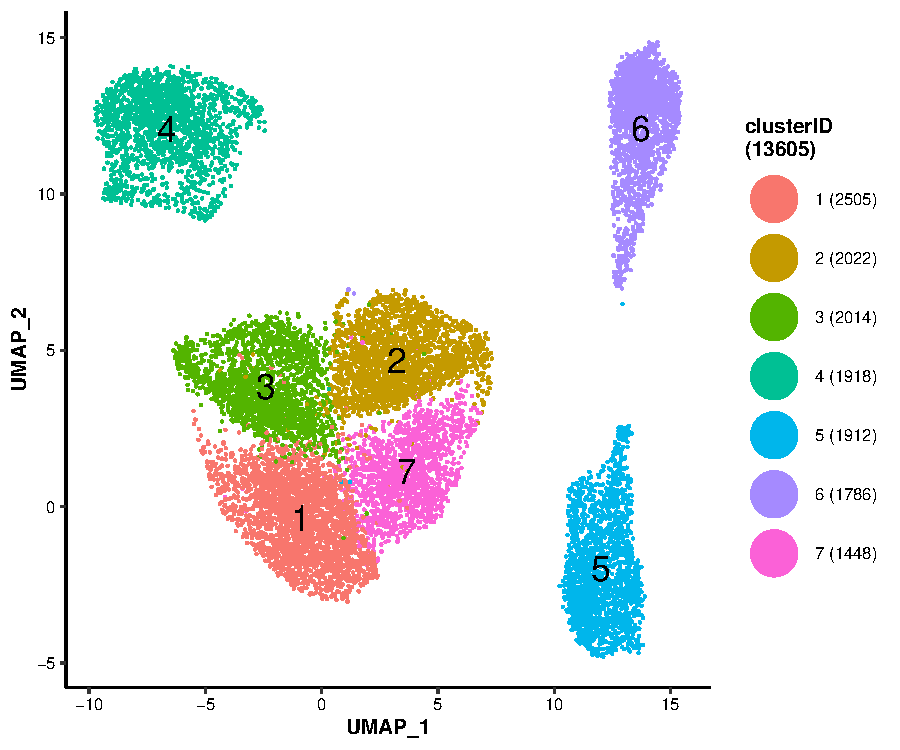
\includegraphics{_main_files/figure-latex/visualize-mica-output-cluster-1} \end{center}

\subsection{Color-coded by true label of cell types}\label{color-coded-by-true-label-of-cell-types}

\begin{Shaded}
\begin{Highlighting}[]
\FunctionTok{MICAplot}\NormalTok{(}\AttributeTok{input\_eset =}\NormalTok{ pbmc14k\_log2cpm.eset, }\AttributeTok{color\_by =} \StringTok{"trueLabel"}\NormalTok{, }\AttributeTok{X =} \StringTok{"UMAP\_1"}\NormalTok{, }\AttributeTok{Y =} \StringTok{"UMAP\_2"}\NormalTok{, }\AttributeTok{point.size =} \FloatTok{0.1}\NormalTok{, }\AttributeTok{fontsize.cluster\_label =} \DecValTok{4}\NormalTok{)}
\end{Highlighting}
\end{Shaded}

\begin{center}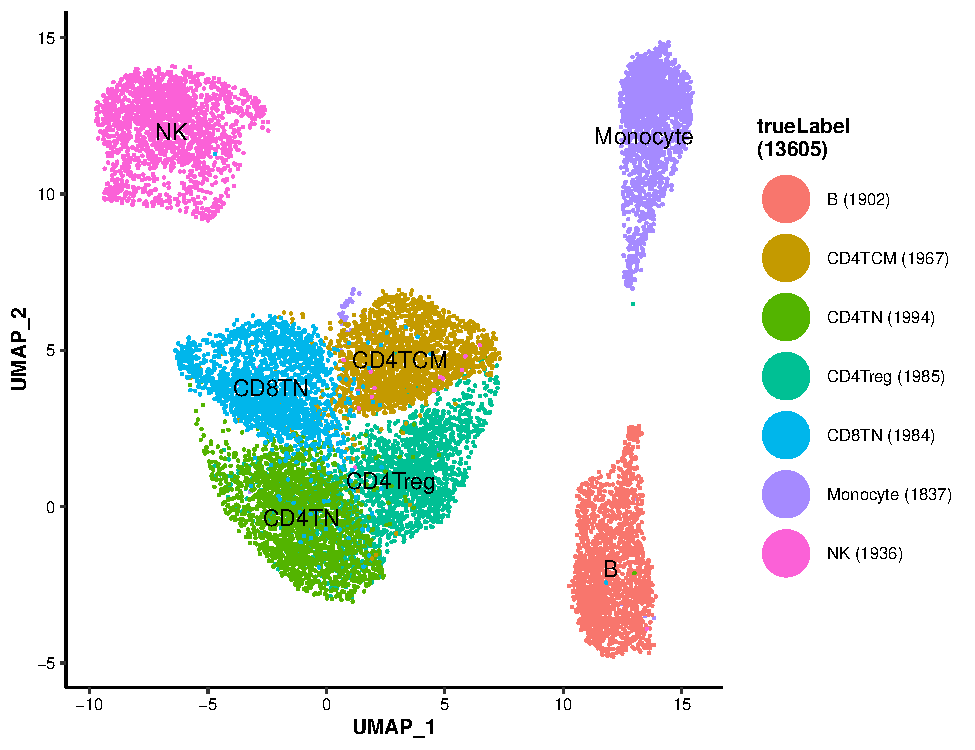
\includegraphics{_main_files/figure-latex/visualize-mica-output-truelabel-1} \end{center}

\subsection{Color-coded by nUMI, for QC purpose}\label{color-coded-by-numi-for-qc-purpose}

\begin{Shaded}
\begin{Highlighting}[]
\FunctionTok{MICAplot}\NormalTok{(}\AttributeTok{input\_eset =}\NormalTok{ pbmc14k\_log2cpm.eset, }\AttributeTok{color\_by =} \StringTok{"nUMI"}\NormalTok{, }\AttributeTok{do.logTransform =} \ConstantTok{TRUE}\NormalTok{, }\AttributeTok{point.size =} \FloatTok{0.1}\NormalTok{)}
\end{Highlighting}
\end{Shaded}

\begin{verbatim}
## The values in "nUMI" have been transformed by log2(value + 1). To turn transformation off, set do.logTransform = FALSE.
\end{verbatim}

\begin{center}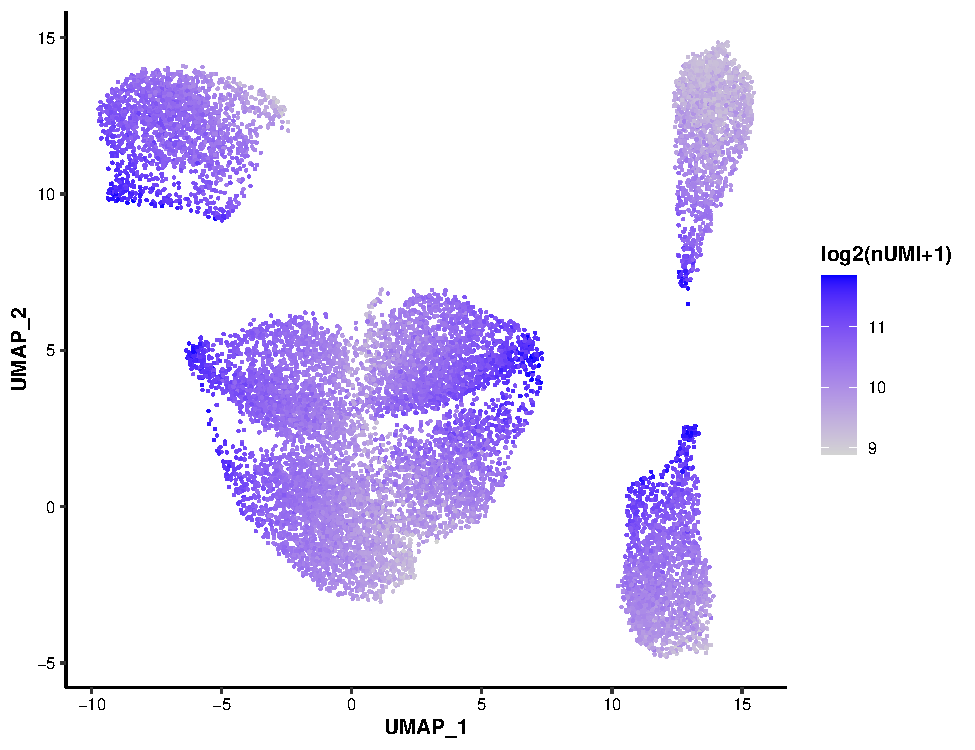
\includegraphics{_main_files/figure-latex/visualize-mica-output-numi-1} \end{center}

\subsection{Color-coded by nFeature, for QC purpose}\label{color-coded-by-nfeature-for-qc-purpose}

\begin{Shaded}
\begin{Highlighting}[]
\FunctionTok{MICAplot}\NormalTok{(}\AttributeTok{input\_eset =}\NormalTok{ pbmc14k\_log2cpm.eset, }\AttributeTok{color\_by =} \StringTok{"nFeature"}\NormalTok{, }\AttributeTok{do.logTransform =} \ConstantTok{TRUE}\NormalTok{, }\AttributeTok{point.size =} \FloatTok{0.1}\NormalTok{)}
\end{Highlighting}
\end{Shaded}

\begin{verbatim}
## The values in "nFeature" have been transformed by log2(value + 1). To turn transformation off, set do.logTransform = FALSE.
\end{verbatim}

\begin{center}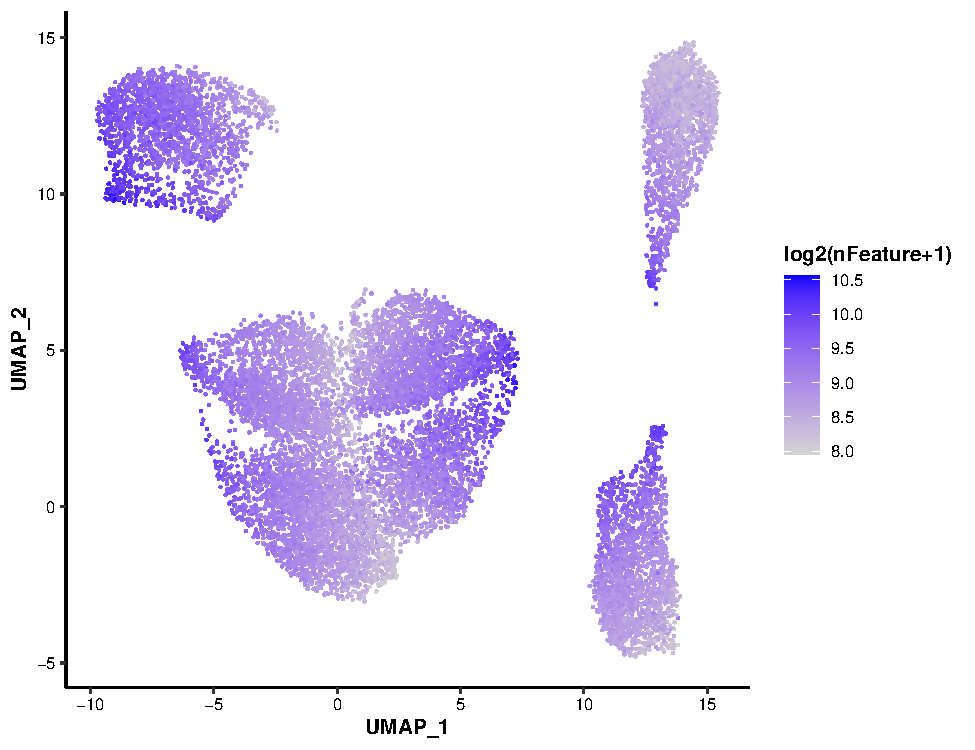
\includegraphics{_main_files/figure-latex/visualize-mica-output-nfeature-1} \end{center}

\subsection{Color-coded by pctMito, for QC purpose}\label{color-coded-by-pctmito-for-qc-purpose}

\begin{Shaded}
\begin{Highlighting}[]
\FunctionTok{MICAplot}\NormalTok{(}\AttributeTok{input\_eset =}\NormalTok{ pbmc14k\_log2cpm.eset, }\AttributeTok{color\_by =} \StringTok{"pctMito"}\NormalTok{, }\AttributeTok{do.logTransform =} \ConstantTok{FALSE}\NormalTok{, }\AttributeTok{point.size =} \FloatTok{0.1}\NormalTok{)}
\end{Highlighting}
\end{Shaded}

\begin{center}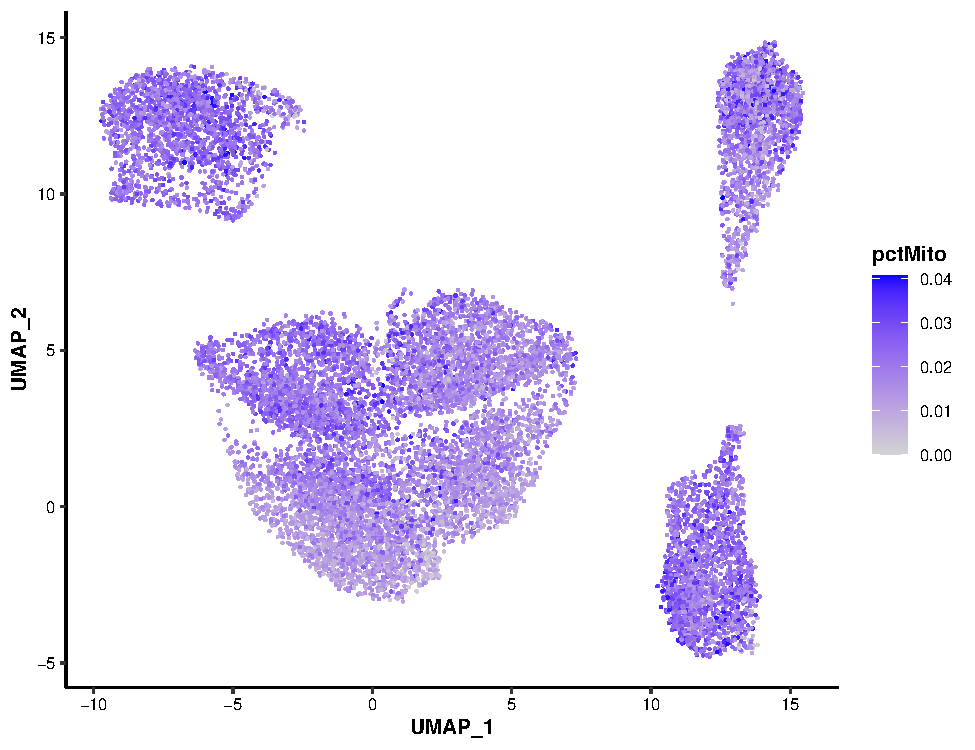
\includegraphics{_main_files/figure-latex/visualize-mica-output-pctmito-1} \end{center}

\chapter{Cell type annotation}\label{cell-type-annotation}

Currently, there are two types of strategies to annotate the clusters: \textbf{supervised} and \textbf{unsupervised}. The \textbf{supervised} methods use a list of known markers of potential cell types curated from somoe existing studies of the same/similar contexts. While in contrast, the \textbf{unsupervised} methods are usually based on the differentially expressed genes. scMINER provide several useful functions to support both types of strategies.

\section{Supervised cell type annotation}\label{supervised-cell-type-annotation}

In the past a few years, the scRNA-seq data has dramatically increased in both quality and quantity. For the majority of tissue types, some existing studies on the same/similar tissue type are most likely available, and from these existing studies, we can figure out a list of candidate cell types to expect and curate a list of markers for each of them. In this case, we know the 7 cell types involved in the dataset, and curated a marker list from some existing PBMCs studies.

\subsection{Annotate using signature scores}\label{annotate-using-signature-scores}

Given a marker list of candidate cell types, scMINER can estimate a signature score, which is mathematically \texttt{the\ weighted\ mean\ of\ the\ expression\ of\ marker\ genes\ involved}, for each candidate cell type across all cell cluster. To do so, you will need to generate a signature table with three columns:

\begin{itemize}
\tightlist
\item
  \texttt{signature\_name}: name of cell types/signatures;
\item
  \texttt{signature\_feature}: markers genes/features of corresponding cell type/signature;
\item
  \texttt{weight}: weight of corresponding maker/feature in corresponding cell type/signature. It ranges from -1 to 1, so both positive and negtive markers are supoorted.
\end{itemize}

\begin{Shaded}
\begin{Highlighting}[]
\DocumentationTok{\#\# Signature table of PBMC14k dataset}
\NormalTok{signature\_table }\OtherTok{\textless{}{-}} \FunctionTok{read.table}\NormalTok{(}\FunctionTok{system.file}\NormalTok{(}\StringTok{"extdata/demo\_pbmc14k/PBMC14k\_signatureTable.txt"}\NormalTok{, }\AttributeTok{package =} \StringTok{"scMINER"}\NormalTok{), }\AttributeTok{header =} \ConstantTok{TRUE}\NormalTok{, }\AttributeTok{sep =} \StringTok{"}\SpecialCharTok{\textbackslash{}t}\StringTok{"}\NormalTok{, }\AttributeTok{quote =} \StringTok{""}\NormalTok{, }\AttributeTok{stringsAsFactors =} \ConstantTok{FALSE}\NormalTok{)}
\FunctionTok{head}\NormalTok{(signature\_table)}
\end{Highlighting}
\end{Shaded}

\begin{verbatim}
##   signature_name signature_feature weight
## 1       Monocyte              CD14      1
## 2       Monocyte               LYZ      1
## 3       Monocyte            S100A8      1
## 4       Monocyte            S100A9      1
## 5       Monocyte           S100A12      1
## 6             NK            FCGR3A      1
\end{verbatim}

With this signature table, \texttt{draw\_bubbleplot()} can estimate the signature scores and visualize them using bubble plot:

\begin{Shaded}
\begin{Highlighting}[]
\DocumentationTok{\#\# Violin plot of marker genes across clusters}
\FunctionTok{draw\_bubbleplot}\NormalTok{(}\AttributeTok{input\_eset =}\NormalTok{ pbmc14k\_log2cpm.eset, }\AttributeTok{signature\_table =}\NormalTok{ signature\_table, }\AttributeTok{group\_by =} \StringTok{"clusterID"}\NormalTok{)}
\end{Highlighting}
\end{Shaded}

\begin{verbatim}
## 31 features of 7 signatures were found in the input eset and will be used in calculation.
\end{verbatim}

\begin{center}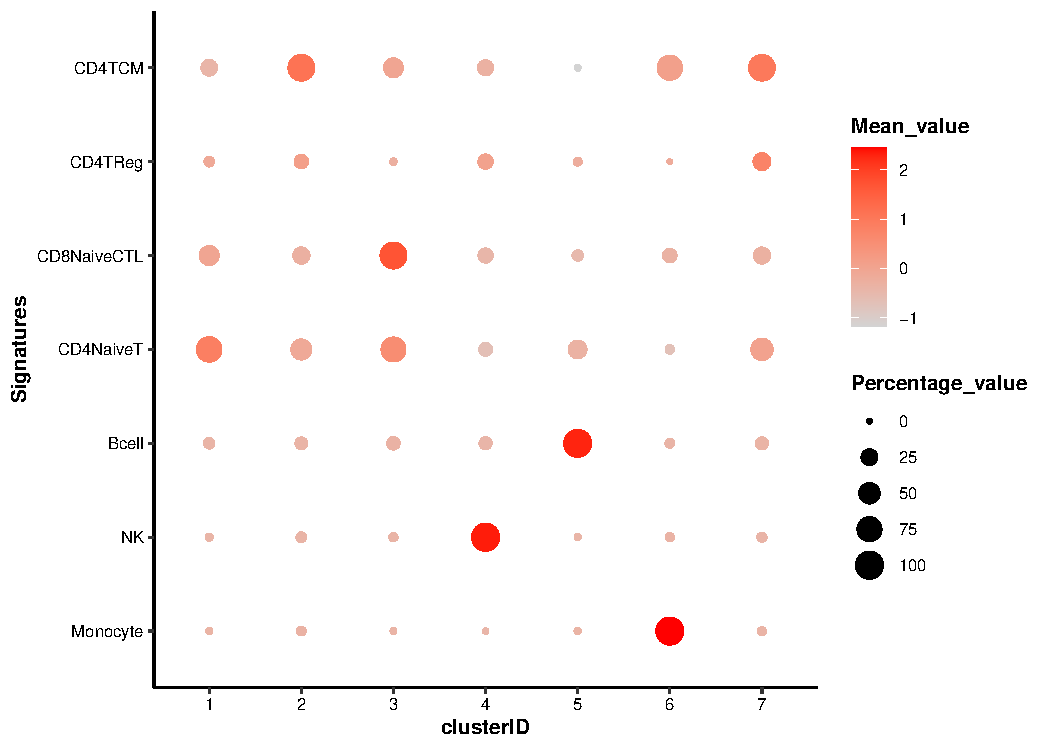
\includegraphics{_main_files/figure-latex/signature-bubble-1} \end{center}

In the bubble plot above, the color of the bubbles is proportional to the mean of signature score, and the size of the bubbles is proportional to the percentage of cells with higher signature score than mean. The cell type of each cluster is clear, except the cluster 7, which shows equally-high signature score of both CD4+ TCM and CD4+ Reg and higher percentage of CD4+ TCM cells.

\subsection{Annotate using individual marker genes}\label{annotate-using-individual-marker-genes}

scMINER also provides a variety of functions to visualize the selected features:

\begin{Shaded}
\begin{Highlighting}[]
\DocumentationTok{\#\# For the demonstration purposes, we picked two well known markers for each of the 7 known cell types, plus "CD3D" and "CD4".}
\NormalTok{genes\_of\_interest }\OtherTok{\textless{}{-}}\FunctionTok{c}\NormalTok{(}\StringTok{"CD14"}\NormalTok{, }\StringTok{"LYZ"}\NormalTok{, }\StringTok{"GZMB"}\NormalTok{, }\StringTok{"NKG7"}\NormalTok{, }\StringTok{"CD19"}\NormalTok{, }\StringTok{"MS4A1"}\NormalTok{, }\StringTok{"CD8A"}\NormalTok{, }\StringTok{"CD8B"}\NormalTok{, }\StringTok{"SELL"}\NormalTok{, }\StringTok{"CCR7"}\NormalTok{, }\StringTok{"IL2RA"}\NormalTok{, }\StringTok{"FOXP3"}\NormalTok{, }\StringTok{"IL7R"}\NormalTok{, }\StringTok{"S100A4"}\NormalTok{, }\StringTok{"CD3D"}\NormalTok{, }\StringTok{"CD4"}\NormalTok{)}
\end{Highlighting}
\end{Shaded}

\subsubsection{feature visualization: violin plot}\label{feature-visualization-violin-plot}

\begin{Shaded}
\begin{Highlighting}[]
\DocumentationTok{\#\# Violin plot of marker genes across clusters}
\FunctionTok{feature\_vlnplot}\NormalTok{(}\AttributeTok{input\_eset =}\NormalTok{ pbmc14k\_log2cpm.eset, }\AttributeTok{features =}\NormalTok{ genes\_of\_interest, }\AttributeTok{group\_by =} \StringTok{"clusterID"}\NormalTok{, }\AttributeTok{ncol =} \DecValTok{4}\NormalTok{)}
\end{Highlighting}
\end{Shaded}

\begin{center}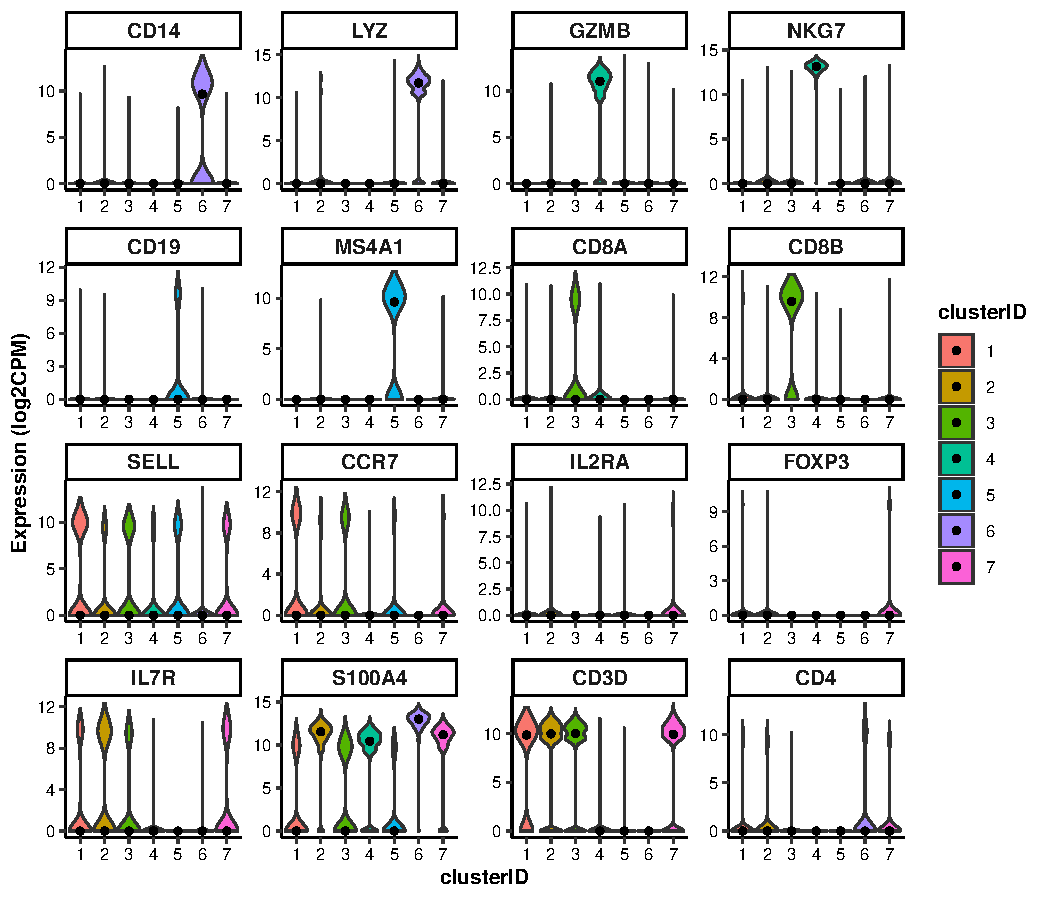
\includegraphics{_main_files/figure-latex/featurePlot-vln-1} \end{center}

\subsubsection{feature visualization: box plot}\label{feature-visualization-box-plot}

\begin{Shaded}
\begin{Highlighting}[]
\DocumentationTok{\#\# Box plot of marker genes across clusters}
\FunctionTok{feature\_boxplot}\NormalTok{(}\AttributeTok{input\_eset =}\NormalTok{ pbmc14k\_log2cpm.eset, }\AttributeTok{features =}\NormalTok{ genes\_of\_interest, }\AttributeTok{group\_by =} \StringTok{"clusterID"}\NormalTok{, }\AttributeTok{ncol =} \DecValTok{4}\NormalTok{)}
\end{Highlighting}
\end{Shaded}

\begin{center}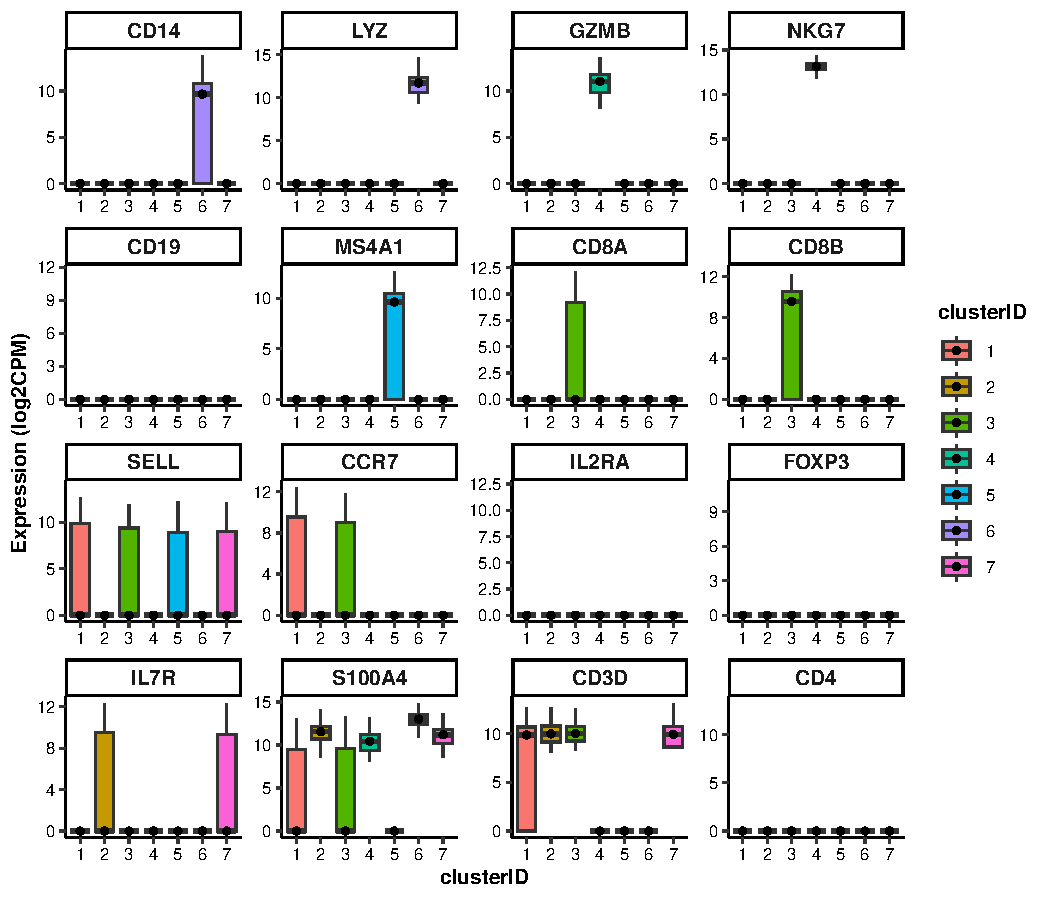
\includegraphics{_main_files/figure-latex/featurePlot-box-1} \end{center}

\subsubsection{feature visualization: scatter plot}\label{feature-visualization-scatter-plot}

\begin{Shaded}
\begin{Highlighting}[]
\DocumentationTok{\#\# UMAP scatter plot of marker genes}
\FunctionTok{feature\_scatterplot}\NormalTok{(}\AttributeTok{input\_eset =}\NormalTok{ pbmc14k\_log2cpm.eset, }\AttributeTok{features =}\NormalTok{ genes\_of\_interest, }\AttributeTok{ncol =} \DecValTok{4}\NormalTok{, }\AttributeTok{location\_x =} \StringTok{"UMAP\_1"}\NormalTok{, }\AttributeTok{location\_y =}  \StringTok{"UMAP\_2"}\NormalTok{, }\AttributeTok{point.size =} \FloatTok{0.5}\NormalTok{, }\AttributeTok{legend.key\_height =} \FloatTok{0.3}\NormalTok{, }\AttributeTok{legend.key\_width =} \FloatTok{0.2}\NormalTok{, }\AttributeTok{fontsize.legend\_title =} \DecValTok{8}\NormalTok{, }\AttributeTok{fontsize.legend\_text =} \DecValTok{6}\NormalTok{, }\AttributeTok{fontsize.axis\_title =} \DecValTok{8}\NormalTok{, }\AttributeTok{legend.position =} \StringTok{"none"}\NormalTok{)}
\end{Highlighting}
\end{Shaded}

\begin{center}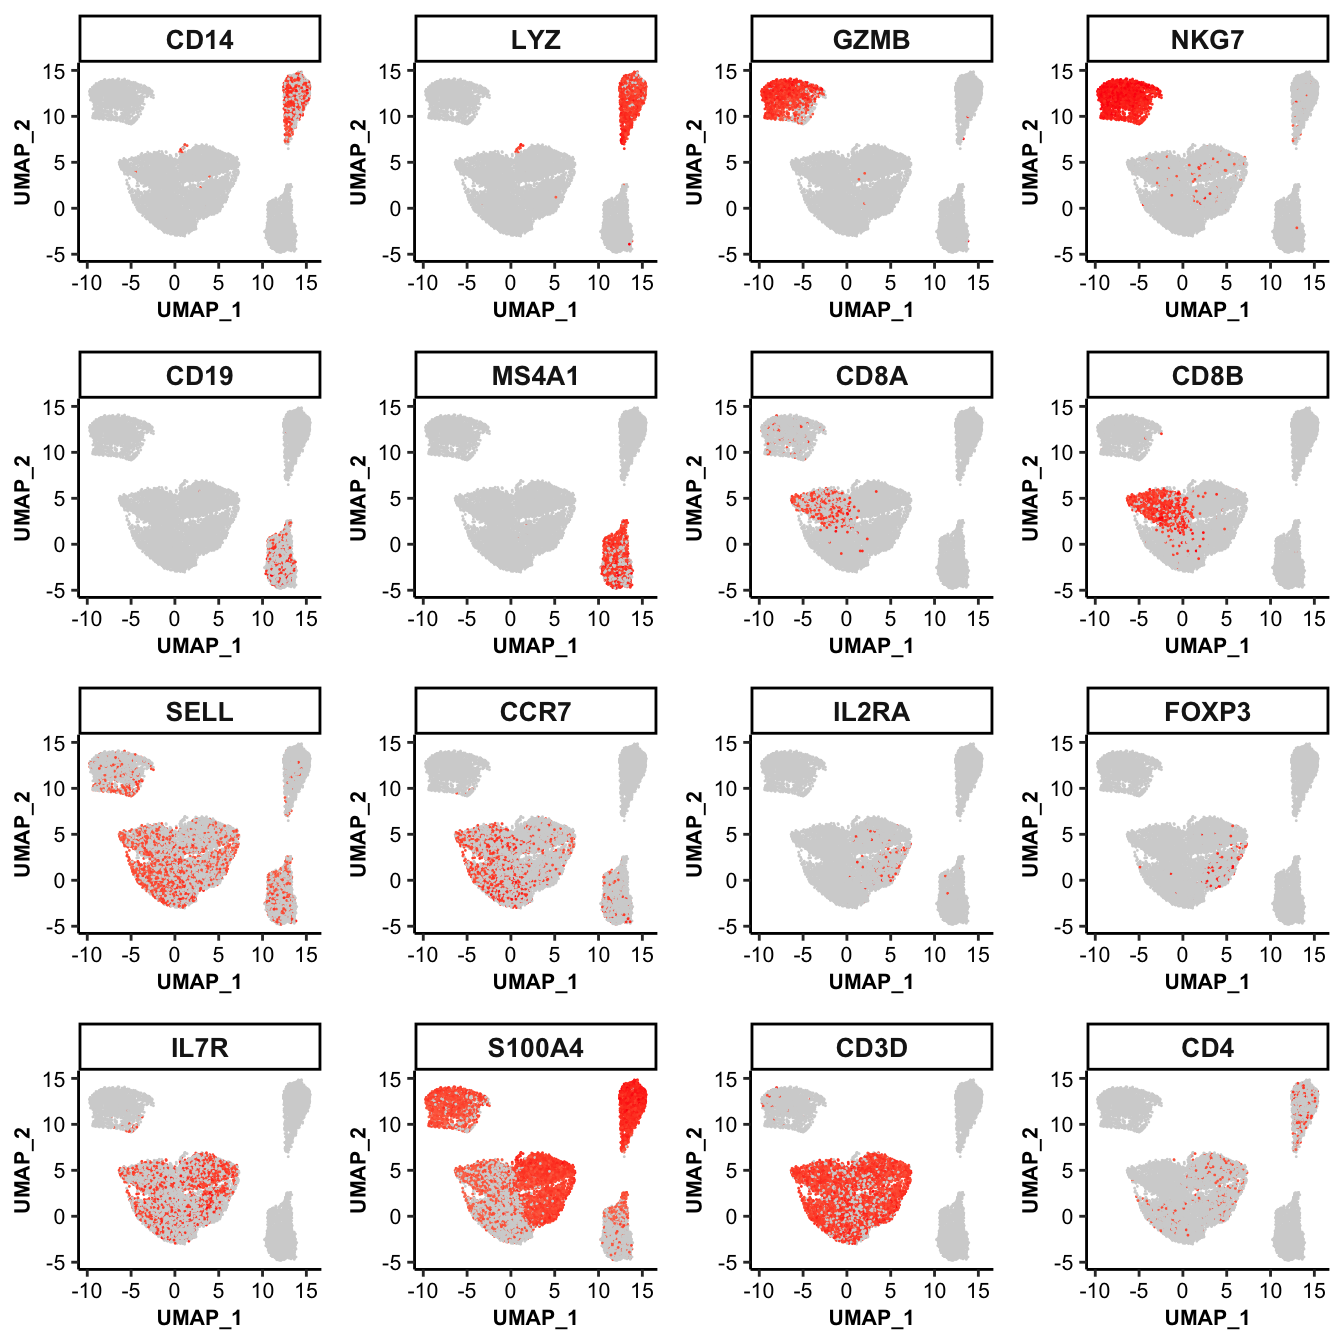
\includegraphics{_main_files/figure-latex/featurePlot-scatter-1} \end{center}

\subsubsection{feature visualization: bubble plot}\label{feature-visualization-bubble-plot}

\begin{Shaded}
\begin{Highlighting}[]
\DocumentationTok{\#\# Bubble plot of marker genes across clusters}
\FunctionTok{feature\_bubbleplot}\NormalTok{(}\AttributeTok{input\_eset =}\NormalTok{ pbmc14k\_log2cpm.eset, }\AttributeTok{features =}\NormalTok{ genes\_of\_interest, }\AttributeTok{group\_by =} \StringTok{"clusterID"}\NormalTok{, }\AttributeTok{xlabel.angle =} \DecValTok{45}\NormalTok{)}
\end{Highlighting}
\end{Shaded}

\begin{center}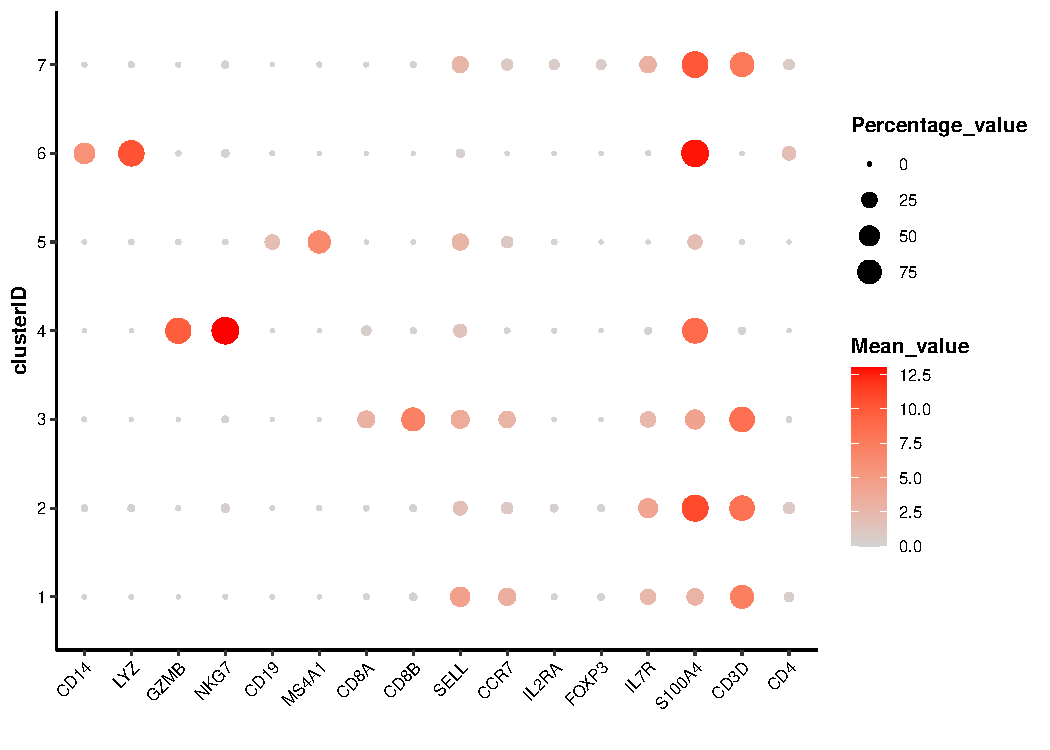
\includegraphics{_main_files/figure-latex/featurePlot-bubble-1} \end{center}

\subsubsection{feature visualization: heatmap}\label{feature-visualization-heatmap}

\begin{Shaded}
\begin{Highlighting}[]
\DocumentationTok{\#\# Heatmap of marker genes across clusters}
\FunctionTok{feature\_heatmap}\NormalTok{(}\AttributeTok{input\_eset =}\NormalTok{ pbmc14k\_log2cpm.eset, }\AttributeTok{features =}\NormalTok{ genes\_of\_interest, }\AttributeTok{group\_by =} \StringTok{"clusterID"}\NormalTok{, }\AttributeTok{scale\_method =} \StringTok{"none"}\NormalTok{, }\AttributeTok{annotation\_columns =} \FunctionTok{c}\NormalTok{(}\StringTok{"trueLabel"}\NormalTok{))}
\end{Highlighting}
\end{Shaded}

\begin{center}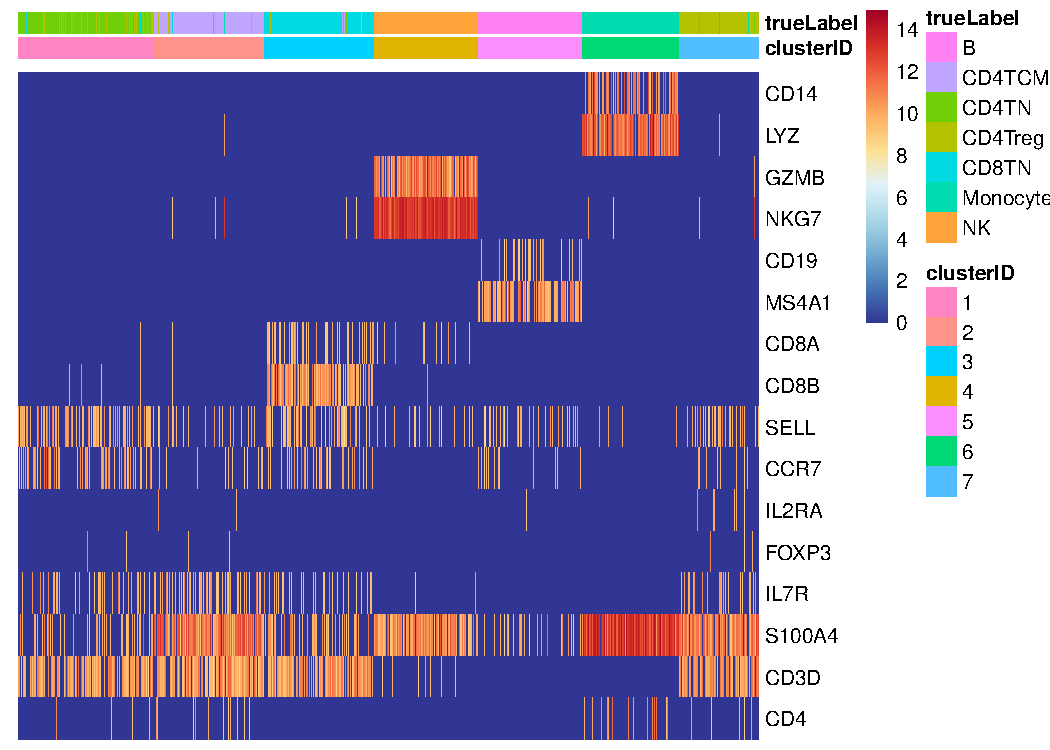
\includegraphics{_main_files/figure-latex/featurePlot-heatmap-1} \end{center}

\section{Unsupervised cell type annotation}\label{unsupervised-cell-type-annotation}

Existing studies in the same or similar contexts are not always available, and there is a significant concern regarding the reliability of reference studies. This reliability largely depends on the expertise of the original authors who defined the markers and assigned the cell types. Therefore, we strongly encourage users to also try unsupervised methods, which can serve as a means of cross-validation.

scMINER provides a function, \texttt{getDE()}, to perform the differential expression analysis and identify the markers of each cluster. The \texttt{getDE()} function supports three different methods to perform the differential expression analysis, \texttt{limma}, \texttt{wilcoxon} and \texttt{t.test}. And it allows the users to define the groups to compare in a flexible way:

\begin{Shaded}
\begin{Highlighting}[]
\DocumentationTok{\#\# 1. To perform differential expression analysis in a 1{-}vs{-}rest manner for all groups}
\NormalTok{de\_res1 }\OtherTok{\textless{}{-}} \FunctionTok{getDE}\NormalTok{(}\AttributeTok{input\_eset =}\NormalTok{ pbmc14k\_log2cpm.eset[}\DecValTok{500}\NormalTok{,], }\AttributeTok{group\_by =} \StringTok{"clusterID"}\NormalTok{, }\AttributeTok{use\_method =} \StringTok{"limma"}\NormalTok{)}
\end{Highlighting}
\end{Shaded}

\begin{verbatim}
## 7 groups were found in group_by column [ clusterID ].
## Since no group was specified, the differential analysis will be conducted among all groups in the group_by column [ clusterID ] in the 1-vs-rest manner.
##   1 / 7 : group 1 ( 1 ) vs the rest...
##   2505 cells were found for g1.
##   11100 cells were found for g0.
##   2 / 7 : group 1 ( 2 ) vs the rest...
##   2022 cells were found for g1.
##   11583 cells were found for g0.
##   3 / 7 : group 1 ( 3 ) vs the rest...
##   2014 cells were found for g1.
##   11591 cells were found for g0.
##   4 / 7 : group 1 ( 4 ) vs the rest...
##   1918 cells were found for g1.
##   11687 cells were found for g0.
##   5 / 7 : group 1 ( 5 ) vs the rest...
##   1912 cells were found for g1.
##   11693 cells were found for g0.
##   6 / 7 : group 1 ( 6 ) vs the rest...
##   1786 cells were found for g1.
##   11819 cells were found for g0.
##   7 / 7 : group 1 ( 7 ) vs the rest...
##   1448 cells were found for g1.
##   12157 cells were found for g0.
\end{verbatim}

\begin{Shaded}
\begin{Highlighting}[]
\FunctionTok{head}\NormalTok{(de\_res1)}
\end{Highlighting}
\end{Shaded}

\begin{verbatim}
##  [1] feature g1_tag  g0_tag  g1_avg  g0_avg  g1_pct  g0_pct  log2FC  Pval   
## [10] FDR     Zscore 
## <0 rows> (or 0-length row.names)
\end{verbatim}

Here is an brief introduction to the results of \texttt{getDE()}:

\begin{itemize}
\tightlist
\item
  \textbf{feature}: feature name;
\item
  \textbf{g1\_tag}: a vector of clusters or subgroups involved in g1, the fore-ground group;
\item
  \textbf{g0\_tag}: a vector of clusters or subgroups involved in g0, the back-ground group;
\item
  \textbf{g1\_avg}: mean of gene expression of cells in g1;
\item
  \textbf{g0\_tag}: mean of gene expression of cells in g0;
\item
  \textbf{g1\_pct}: percentage of cells expressing the corresponding genes in group 1;
\item
  \textbf{g0\_pct}: percentage of cells expressing the corresponding genes in group 0;
\item
  \textbf{log2FC}: log2Fold change of gene expression between g1 and g0;
\item
  \textbf{Pval}: P values of g1-g0 comparison;
\item
  \textbf{FDR}: FDR of g1-g0 comparison;
\item
  \textbf{Zscore}: Z score of g1-g0 comparison, signed by \texttt{log2FC};
\end{itemize}

\begin{Shaded}
\begin{Highlighting}[]
\DocumentationTok{\#\# 2. To perform differential expression analysis in a 1{-}vs{-}rest manner for one specific group}
\NormalTok{de\_res2 }\OtherTok{\textless{}{-}} \FunctionTok{getDE}\NormalTok{(}\AttributeTok{input\_eset =}\NormalTok{ pbmc14k\_log2cpm.eset, }\AttributeTok{group\_by =} \StringTok{"clusterID"}\NormalTok{, }\AttributeTok{g1 =} \FunctionTok{c}\NormalTok{(}\StringTok{"1"}\NormalTok{), }\AttributeTok{use\_method =} \StringTok{"limma"}\NormalTok{)}

\DocumentationTok{\#\# 3. To perform differential expression analysis in a rest{-}vs{-}1 manner for one specific group}
\NormalTok{de\_res3 }\OtherTok{\textless{}{-}} \FunctionTok{getDE}\NormalTok{(}\AttributeTok{input\_eset =}\NormalTok{ pbmc14k\_log2cpm.eset, }\AttributeTok{group\_by =} \StringTok{"clusterID"}\NormalTok{, }\AttributeTok{g0 =} \FunctionTok{c}\NormalTok{(}\StringTok{"1"}\NormalTok{), }\AttributeTok{use\_method =} \StringTok{"limma"}\NormalTok{)}

\DocumentationTok{\#\# 4. To perform differential expression analysis in a 1{-}vs{-}1 manner for any two groups}
\NormalTok{de\_res4 }\OtherTok{\textless{}{-}} \FunctionTok{getDE}\NormalTok{(}\AttributeTok{input\_eset =}\NormalTok{ pbmc14k\_log2cpm.eset, }\AttributeTok{group\_by =} \StringTok{"clusterID"}\NormalTok{, }\AttributeTok{g1 =} \FunctionTok{c}\NormalTok{(}\StringTok{"1"}\NormalTok{), }\AttributeTok{g0 =} \FunctionTok{c}\NormalTok{(}\StringTok{"3"}\NormalTok{), }\AttributeTok{use\_method =} \StringTok{"limma"}\NormalTok{)}
\end{Highlighting}
\end{Shaded}

scMINER also provides a function, \texttt{getTopFeatures()}, to easily extract the group-specific markers from the differential expression result:

\begin{Shaded}
\begin{Highlighting}[]
\NormalTok{cluster\_markers }\OtherTok{\textless{}{-}} \FunctionTok{getTopFeatures}\NormalTok{(}\AttributeTok{input\_table =}\NormalTok{ de\_res1, }\AttributeTok{number =} \DecValTok{10}\NormalTok{, }\AttributeTok{group\_by =} \StringTok{"g1\_tag"}\NormalTok{, }\AttributeTok{sort\_by =} \StringTok{"log2FC"}\NormalTok{, }\AttributeTok{sort\_decreasing =} \ConstantTok{TRUE}\NormalTok{)}
\FunctionTok{dim}\NormalTok{(cluster\_markers)}
\end{Highlighting}
\end{Shaded}

\begin{verbatim}
## [1]  0 11
\end{verbatim}

\begin{Shaded}
\begin{Highlighting}[]
\FunctionTok{head}\NormalTok{(cluster\_markers)}
\end{Highlighting}
\end{Shaded}

\begin{verbatim}
##  [1] feature g1_tag  g0_tag  g1_avg  g0_avg  g1_pct  g0_pct  log2FC  Pval   
## [10] FDR     Zscore 
## <0 rows> (or 0-length row.names)
\end{verbatim}

\section{Add cell type annotations to SparseExpressionSet object}\label{add-cell-type-annotations-to-sparseexpressionset-object}

Based on the supervised and unsupervised methods, we have annotated the cell types for each cluster. To add the cell type annotation information into the sparse eset object:

\begin{Shaded}
\begin{Highlighting}[]
\NormalTok{celltype\_map }\OtherTok{\textless{}{-}} \FunctionTok{c}\NormalTok{(}\StringTok{\textasciigrave{}}\AttributeTok{1}\StringTok{\textasciigrave{}}\OtherTok{=}\StringTok{"CD4TN"}\NormalTok{, }\StringTok{\textasciigrave{}}\AttributeTok{2}\StringTok{\textasciigrave{}}\OtherTok{=}\StringTok{"CD4TCM"}\NormalTok{, }\StringTok{\textasciigrave{}}\AttributeTok{3}\StringTok{\textasciigrave{}}\OtherTok{=}\StringTok{"CD8TN"}\NormalTok{, }\StringTok{\textasciigrave{}}\AttributeTok{4}\StringTok{\textasciigrave{}}\OtherTok{=}\StringTok{"NK"}\NormalTok{, }\StringTok{\textasciigrave{}}\AttributeTok{5}\StringTok{\textasciigrave{}}\OtherTok{=}\StringTok{"B"}\NormalTok{, }\StringTok{\textasciigrave{}}\AttributeTok{6}\StringTok{\textasciigrave{}}\OtherTok{=}\StringTok{"Monocyte"}\NormalTok{, }\StringTok{\textasciigrave{}}\AttributeTok{7}\StringTok{\textasciigrave{}}\OtherTok{=}\StringTok{"CD4Treg"}\NormalTok{)}
\NormalTok{pbmc14k\_log2cpm.eset}\SpecialCharTok{$}\NormalTok{cell\_type }\OtherTok{\textless{}{-}} \FunctionTok{as.character}\NormalTok{(celltype\_map[pbmc14k\_log2cpm.eset}\SpecialCharTok{$}\NormalTok{clusterID])}
\FunctionTok{head}\NormalTok{(}\FunctionTok{pData}\NormalTok{(pbmc14k\_log2cpm.eset))}
\end{Highlighting}
\end{Shaded}

\begin{verbatim}
##                trueLabel_full trueLabel projectID nUMI nFeature    pctMito
## CACTTTGACGCAAT CD14+ Monocyte  Monocyte   PBMC14k  764      354 0.01832461
## GTTACGGAAACGAA CD14+ Monocyte  Monocyte   PBMC14k  956      442 0.01569038
## CACTTATGAGTCGT CD14+ Monocyte  Monocyte   PBMC14k  629      323 0.02066773
## GCATGTGATTCTGT CD14+ Monocyte  Monocyte   PBMC14k  875      427 0.02628571
## TAGAATACGTATCG CD14+ Monocyte  Monocyte   PBMC14k 1060      445 0.03207547
## CAAGAAGACCCTCA CD14+ Monocyte  Monocyte   PBMC14k  849      384 0.01531213
##                pctSpikeIn         CellID   UMAP_1   UMAP_2 clusterID cell_type
## CACTTTGACGCAAT          0 CACTTTGACGCAAT 14.91650 13.04096         6  Monocyte
## GTTACGGAAACGAA          0 GTTACGGAAACGAA 14.57031 10.27093         6  Monocyte
## CACTTATGAGTCGT          0 CACTTATGAGTCGT 14.28869 13.61674         6  Monocyte
## GCATGTGATTCTGT          0 GCATGTGATTCTGT 14.12546 13.36319         6  Monocyte
## TAGAATACGTATCG          0 TAGAATACGTATCG 14.91227 11.19407         6  Monocyte
## CAAGAAGACCCTCA          0 CAAGAAGACCCTCA 15.34154 12.25821         6  Monocyte
\end{verbatim}

The \texttt{draw\_barplot()} function can visualize the cell composition of self-defined groups. We can use it to show the purity of MICA clusters:

\begin{Shaded}
\begin{Highlighting}[]
\DocumentationTok{\#\# Violin plot of marker genes across clusters}
\FunctionTok{draw\_barplot}\NormalTok{(}\AttributeTok{input\_eset =}\NormalTok{ pbmc14k\_log2cpm.eset, }\AttributeTok{group\_by =} \StringTok{"cell\_type"}\NormalTok{, }\AttributeTok{color\_by =} \StringTok{"trueLabel\_full"}\NormalTok{, }\AttributeTok{xlabel.angle =} \DecValTok{45}\NormalTok{)}
\end{Highlighting}
\end{Shaded}

\begin{center}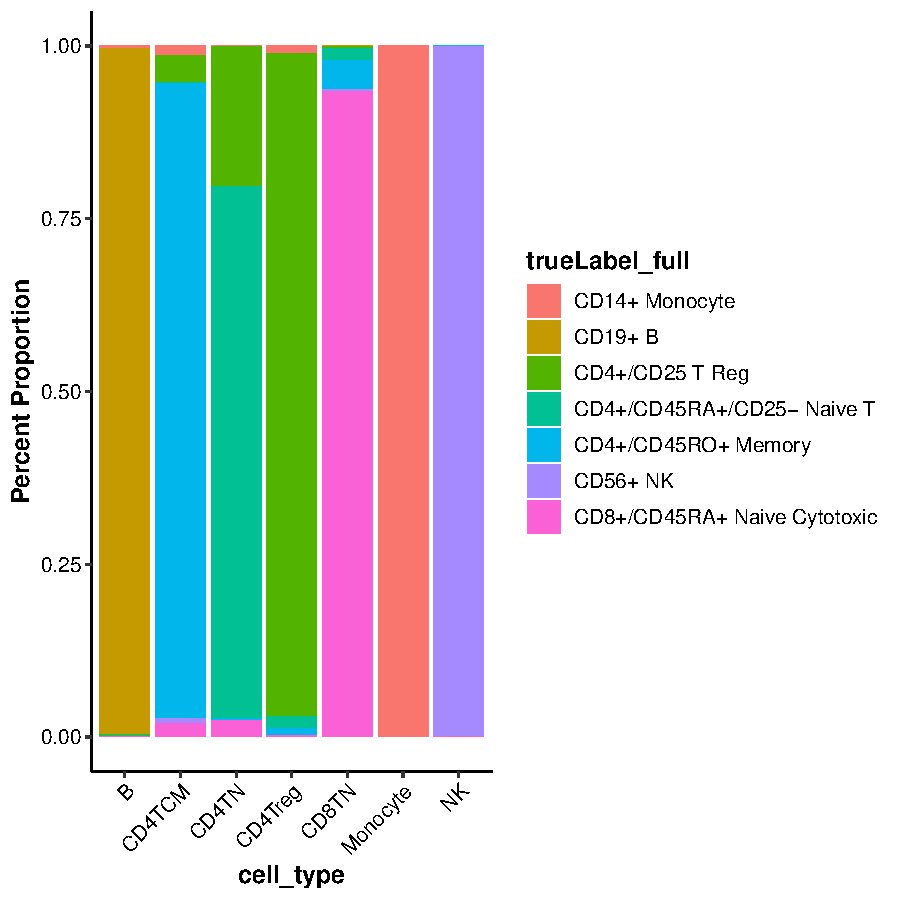
\includegraphics{_main_files/figure-latex/group-barplot-1} \end{center}

Don't forget to save the SparseEset object after the cell type annotation added.

\begin{Shaded}
\begin{Highlighting}[]
\FunctionTok{saveRDS}\NormalTok{(pbmc14k\_log2cpm.eset, }\AttributeTok{file =} \StringTok{"/your{-}path/PBMC14k/DATA/pbmc14k\_log2CPM\_annotated.rds"}\NormalTok{)}
\end{Highlighting}
\end{Shaded}

\chapter{Network inference}\label{network-inference}

\href{https://academic.oup.com/bioinformatics/article/35/12/2165/5156064}{SJARACNe} is a scalable software tool for gene network reverse engineering from big data. As an improved implementation of the ARACNe, SJARACNe achieves a dramatic improvement in computational performance in both time and memory usage and implements new features while preserving the network inference accuracy of the original algorithm.

Similar to MICA, SJARACNe is also a component of scMINER framework, and can work seamlessly with the SparseExpressionSet object. The input for MICA can be easily generated from the SparseExpressionSet object by \texttt{generateSJARACNeInput()}, and the output of SJARACNe, the networks, can be effortlessly assessed by \texttt{drawNetworkQC()} and directly taken for driver activity estimation by \texttt{getActivity\_individual()} and \texttt{getActivity\_inBatch()}.

\section{Generate SJARACNe input files}\label{generate-sjaracne-input-files}

The network inference is usually conducted in a \textbf{cluster-} or \textbf{cell type-specific} basis. Given the column names for grouping, \texttt{generateSJARACNeInput()} will create a folder for each group named by the group label.

\textbf{\emph{IMPORTANT NOTE}}: Any \textbf{illegal characters in path} in group labels may cause issues in subsequent analysis. To avoid it, scMINER only accept letters(A-Za-z), numbers(0-9), underscores('\_`) and periods('.').

In this case, the true labels of cell type are available, so we use them to define the groups for network inference.

\begin{Shaded}
\begin{Highlighting}[]
\DocumentationTok{\#\# Columns with any illegal characters can not be used for groupping}
\FunctionTok{generateSJARACNeInput}\NormalTok{(}\AttributeTok{input\_eset =}\NormalTok{ pbmc14k\_log2cpm.eset, }\AttributeTok{group\_name =} \StringTok{"trueLabel"}\NormalTok{, }\AttributeTok{sjaracne\_dir =} \StringTok{"/work{-}path/PBMC14k/SJARACNe"}\NormalTok{, }\AttributeTok{species\_type =} \StringTok{"hg"}\NormalTok{, }\AttributeTok{driver\_type =} \StringTok{"TF\_SIG"}\NormalTok{, }\AttributeTok{downSample\_N =} \ConstantTok{NULL}\NormalTok{)}
\end{Highlighting}
\end{Shaded}

For big datasets, \texttt{generateSJARACNeInput()} provides an argument, \texttt{downSample\_N}, to allow users to down sample size of each group. The default value of \texttt{downSample\_N} is 1,000, any group with \textgreater= 1,000 cells will be down-sample to 1,000.

\begin{Shaded}
\begin{Highlighting}[]
\DocumentationTok{\#\# one folder for each group}
\FunctionTok{list.dirs}\NormalTok{(}\FunctionTok{system.file}\NormalTok{(}\StringTok{"extdata/demo\_pbmc14k/PBMC14k/SJARACNe"}\NormalTok{, }\AttributeTok{package =} \StringTok{"scMINER"}\NormalTok{), }\AttributeTok{full.names =} \ConstantTok{FALSE}\NormalTok{, }\AttributeTok{recursive =} \ConstantTok{FALSE}\NormalTok{)}
\end{Highlighting}
\end{Shaded}

\begin{verbatim}
## [1] "B"        "CD4TCM"   "CD4TN"    "CD4Treg"  "CD8TN"    "Monocyte" "NK"
\end{verbatim}

\begin{Shaded}
\begin{Highlighting}[]
\DocumentationTok{\#\# file structure of each folder}
\FunctionTok{list.files}\NormalTok{(}\FunctionTok{system.file}\NormalTok{(}\StringTok{"extdata/demo\_pbmc14k/PBMC14k/SJARACNe/B"}\NormalTok{, }\AttributeTok{package =} \StringTok{"scMINER"}\NormalTok{), }\AttributeTok{full.names =} \ConstantTok{FALSE}\NormalTok{, }\AttributeTok{recursive =} \ConstantTok{TRUE}\NormalTok{, }\AttributeTok{include.dirs =} \ConstantTok{FALSE}\NormalTok{, }\AttributeTok{pattern =} \StringTok{"[\^{}consensus\_network\_ncol\_.txt]"}\NormalTok{)}
\end{Highlighting}
\end{Shaded}

\begin{verbatim}
## [1] "B.8572_1902.exp.txt"     "config_cwlexec.json"    
## [3] "runSJARACNe.sh"          "SIG/B.4148_1902.sig.txt"
## [5] "TF/B.835_1902.tf.txt"
\end{verbatim}

The standard input files of SJARACNe, for each group, include:

\begin{itemize}
\tightlist
\item
  a ``\textbf{\texttt{.exp.txt}}'' file: a tab-separated genes/transcripts/proteins by cells/samples expression matrix with the first two columns being ID and symbol.
\item
  a ``\textbf{\texttt{TF}}'' folder containing a ``\textbf{\texttt{.tf.txt}}'' file: a list of significant gene/transcript/protein IDs of TF drivers.
\item
  a ``\textbf{\texttt{SIG}}'' folder containing a ``\textbf{\texttt{.sig.txt}}'' file: a list of significant gene/transcript/protein IDs of SIG drivers.
\item
  a bash script (\textbf{\texttt{runSJARACNe.sh}}) to run SJARACNe. Further modification is needed to run it.
\item
  a json file (\textbf{\texttt{config\_cwlexec.json}}) containing parameters to run SJARACNe.
\end{itemize}

Usually, the ground truth of cell types is not available. Then the \textbf{cluster labels}, or \textbf{cell type annotations of the clusters}, can be used for grouping in network rewiring, since it's expected that cells with same cluster label/annotated cell type are of similar gene expression profiles. To generate from annotated cell types, you can run:

\begin{Shaded}
\begin{Highlighting}[]
\FunctionTok{generateSJARACNeInput}\NormalTok{(}\AttributeTok{input\_eset =}\NormalTok{ pbmc14k\_log2cpm.eset, }\AttributeTok{group\_name =} \StringTok{"cell\_type"}\NormalTok{, }\AttributeTok{sjaracne\_dir =} \StringTok{"/work{-}path/PBMC14k/SJARACNe/bycelltype"}\NormalTok{, }\AttributeTok{species\_type =} \StringTok{"hg"}\NormalTok{, }\AttributeTok{driver\_type =} \StringTok{"TF\_SIG"}\NormalTok{)}
\end{Highlighting}
\end{Shaded}

\section{Run SJARACNe}\label{run-sjaracne}

By default, the \texttt{generateSJARACNeInput()} function also generates a \texttt{runSJARACNe.sh} file in the folder of each group. This file much be modified before you can run it:

\begin{itemize}
\tightlist
\item
  \textbf{removed unneeded lines}: There are usually 4 lines in this file: the lines starting with ``sjaracne lsf'' are the command lines to run on IBM LSF cluster, while the lines starting with ``sjaracne local'' are the command lines runing on a single machine (Linux/OSX). Please select the lines based on your situation and remove the others.
\item
  \textbf{-n}: number of bootstrap networks to generate. Default: 100.
\item
  \textbf{-pc}: p value threshold to select edges in building consensus network. Default: e-2 for single-cell data, e-3 for meta-cell data, and e-5 for bulk sample data.
  Please use ``sjaracne lsf -h'' or ``sjaracne local -h'' to check more details of arguments available in SJARACNe.
\end{itemize}

There is another file, \texttt{config\_cwlexec.json}, available in the folder. It contains the information (e.g.~memory request for each step of SJARACNe run) used for LSF job submission. This file is only needed for LSF runs and the default values works well in most cases. If you are running SJARACNe on a big dataset, you may need to request more memory from it.

In this case, we use LSF to run the SJARACNe:

\begin{Shaded}
\begin{Highlighting}[]
\CommentTok{\#\# let\textquotesingle{}s use B cell as an example}
\CommentTok{\# for TF}
\ExtensionTok{sjaracne}\NormalTok{ lsf }\AttributeTok{{-}e}\NormalTok{ /work{-}path/PBMC14k/SJARACNe/B/B.8572\_1902.exp.txt }\AttributeTok{{-}g}\NormalTok{ /work{-}path/PBMC14k/SJARACNe/B/TF/B.835\_1902.tf.txt }\AttributeTok{{-}o}\NormalTok{ /work{-}path/PBMC14k/SJARACNe/B/TF/bt100\_pc001 }\AttributeTok{{-}n}\NormalTok{ 100 }\AttributeTok{{-}pc}\NormalTok{ 0.01 }\AttributeTok{{-}j}\NormalTok{ /work{-}path/PBMC14k/SJARACNe/B/config\_cwlexec.json}

\CommentTok{\# for SIG}
\ExtensionTok{sjaracne}\NormalTok{ lsf }\AttributeTok{{-}e}\NormalTok{ /work{-}path/PBMC14k/SJARACNe/B/B.8572\_1902.exp.txt }\AttributeTok{{-}g}\NormalTok{ /work{-}path/PBMC14k/SJARACNe/B/SIG/B.4148\_1902.sig.txt }\AttributeTok{{-}o}\NormalTok{ /work{-}path/PBMC14k/SJARACNe/B/SIG/bt100\_pc001 }\AttributeTok{{-}n}\NormalTok{ 100 }\AttributeTok{{-}pc}\NormalTok{ 0.01 }\AttributeTok{{-}j}\NormalTok{ /work{-}path/PBMC14k/SJARACNe/B/config\_cwlexec.json}
\end{Highlighting}
\end{Shaded}

We created a folder named ``\textbf{bt100\_pc001}'' in both TF and SIG folders of each group, to save the networks generated under \textbf{100 bootstraps} (\texttt{-n\ 100}) and \textbf{0.01 consensus p value} (\texttt{-pc\ 0.01}).

To run SJARACNe on a local machine:

\begin{Shaded}
\begin{Highlighting}[]
\CommentTok{\#\# let\textquotesingle{}s use B cell as an example}
\CommentTok{\# for TF}
\ExtensionTok{sjaracne}\NormalTok{ local }\AttributeTok{{-}e}\NormalTok{ /work{-}path/PBMC14k/SJARACNe/B/B.8572\_1902.exp.txt }\AttributeTok{{-}g}\NormalTok{ /work{-}path/PBMC14k/SJARACNe/B/TF/B.835\_1902.tf.txt }\AttributeTok{{-}o}\NormalTok{ /work{-}path/PBMC14k/SJARACNe/B/TF/bt100\_pc001 }\AttributeTok{{-}n}\NormalTok{ 100 }\AttributeTok{{-}pc}\NormalTok{ 0.01}

\CommentTok{\# for SIG}
\ExtensionTok{sjaracne}\NormalTok{ local }\AttributeTok{{-}e}\NormalTok{ /work{-}path/PBMC14k/SJARACNe/B/B.8572\_1902.exp.txt }\AttributeTok{{-}g}\NormalTok{ /work{-}path/PBMC14k/SJARACNe/B/SIG/B.4148\_1902.sig.txt }\AttributeTok{{-}o}\NormalTok{ /work{-}path/PBMC14k/SJARACNe/B/SIG/bt100\_pc001 }\AttributeTok{{-}n}\NormalTok{ 100 }\AttributeTok{{-}pc}\NormalTok{ 0.01}
\end{Highlighting}
\end{Shaded}

\section{Assess the quality of networks}\label{assess-the-quality-of-networks}

\subsection{Introduction to the network file by SJARACNe}\label{introduction-to-the-network-file-by-sjaracne}

The core output of SJARACNe is the network file named \texttt{consensus\_network\_ncol\_.txt}. It contains 9 columns:

\begin{itemize}
\tightlist
\item
  \textbf{source}: ID of the source gene, can be the gene symbol;
\item
  \textbf{target}: ID of the target gene, can be the gene symbol;
\item
  \textbf{source.symbol}: symbol of the source gene;
\item
  \textbf{target.symbol}: symbol of the target gene;
\item
  \textbf{MI}: mutual information of source-gene pair;
\item
  \textbf{pearson}: Pearson correlation coefficient, {[}-1,1{]}
\item
  \textbf{pearson}: Spearman correlation coefficient, {[}-1,1{]}
\item
  \textbf{slope}: slop of the regression line, returned by \texttt{stats.linregression()}
\item
  \textbf{p.value}: p-value for a hypothesis test whose null hypothesis is that the slope is zero, using Wald Test with t-distribution of the test statistic
\end{itemize}

\begin{Shaded}
\begin{Highlighting}[]
\NormalTok{network\_format }\OtherTok{\textless{}{-}} \FunctionTok{read.table}\NormalTok{(}\FunctionTok{system.file}\NormalTok{(}\StringTok{"extdata/demo\_pbmc14k/PBMC14k/SJARACNe/B/TF/bt100\_pc001/consensus\_network\_ncol\_.txt"}\NormalTok{, }\AttributeTok{package =} \StringTok{"scMINER"}\NormalTok{),}
                             \AttributeTok{header =}\NormalTok{ T, }\AttributeTok{sep =} \StringTok{"}\SpecialCharTok{\textbackslash{}t}\StringTok{"}\NormalTok{, }\AttributeTok{quote =} \StringTok{""}\NormalTok{, }\AttributeTok{stringsAsFactors =}\NormalTok{ F)}
\FunctionTok{head}\NormalTok{(network\_format)}
\end{Highlighting}
\end{Shaded}

\begin{verbatim}
##   source     target source.symbol target.symbol     MI pearson spearman   slope
## 1   AATF      ACBD3          AATF         ACBD3 0.0509 -0.0310  -0.0311 -0.0193
## 2   AATF       ADD3          AATF          ADD3 0.0486  0.0228   0.0258  0.0307
## 3   AATF        AES          AATF           AES 0.0511  0.0311   0.0289  0.0668
## 4   AATF     AKR7A2          AATF        AKR7A2 0.0498  0.0319   0.0366  0.0421
## 5   AATF AL928768.3          AATF    AL928768.3 0.0447  0.0247   0.0293  0.0335
## 6   AATF       ALG8          AATF          ALG8 0.0479  0.0358   0.0373  0.0234
##   p.value
## 1  0.1761
## 2  0.3204
## 3  0.1756
## 4  0.1646
## 5  0.2815
## 6  0.1183
\end{verbatim}

\subsection{Generate network QC report}\label{generate-network-qc-report}

There is no simple standards to tell the reliability of networks. Empirically, a network with \textbf{50-300} target size is good. scMINER provides a function, \texttt{drawNetworkQC()}, to quickly assess the quality of networks in batch.

\begin{Shaded}
\begin{Highlighting}[]
\NormalTok{network\_stats }\OtherTok{\textless{}{-}} \FunctionTok{drawNetworkQC}\NormalTok{(}\AttributeTok{sjaracne\_dir =} \StringTok{"/work{-}path/PBMC14K/SJARACNe"}\NormalTok{, }\AttributeTok{generate\_html =} \ConstantTok{FALSE}\NormalTok{) }\CommentTok{\# Set \textasciigrave{}generate\_html = TRUE\textasciigrave{} to generate html{-}format QC report for each network file}
\end{Highlighting}
\end{Shaded}

\begin{Shaded}
\begin{Highlighting}[]
\DocumentationTok{\#\# The network QC statistics table is saved seperately, for demonstration purposes.}
\NormalTok{network\_stats }\OtherTok{\textless{}{-}} \FunctionTok{readRDS}\NormalTok{(}\FunctionTok{system.file}\NormalTok{(}\StringTok{"extdata/demo\_pbmc14k/PBMC14k/SJARACNe/network\_stats.rds"}\NormalTok{, }\AttributeTok{package =} \StringTok{"scMINER"}\NormalTok{))}
\FunctionTok{head}\NormalTok{(network\_stats)}
\end{Highlighting}
\end{Shaded}

\begin{verbatim}
##              network_tag network_node network_edge driver_count targetSize_mean
## 1      B.SIG.bt100_pc001         8572       391889         4148        94.47662
## 2       B.TF.bt100_pc001         8572        95341          835       114.18084
## 3 CD4TCM.SIG.bt100_pc001         8660       382153         4209        90.79425
## 4  CD4TCM.TF.bt100_pc001         8660        94319          838       112.55251
## 5  CD4TN.SIG.bt100_pc001         8612       401658         4180        96.09043
## 6   CD4TN.TF.bt100_pc001         8612        95152          831       114.50301
##   targetSize_median targetSize_minimum targetSize_maximum
## 1              94.0                 33                396
## 2              96.0                 64                913
## 3              91.0                 31                281
## 4              95.5                 60                689
## 5              95.0                 43                303
## 6              99.0                 64                743
##                                                                                                                                                                                               network_path
## 1      /Volumes/projects/scRNASeq/yu3grp/scMINER/NG_Revision/QPan/scminer_R/Datasets/PBMC14K/SJARACNe/B/SIG/bt100_pc001/sjaracne_workflow-df798096-8dee-4baf-8f70-891c689dc769/consensus_network_ncol_.txt
## 2       /Volumes/projects/scRNASeq/yu3grp/scMINER/NG_Revision/QPan/scminer_R/Datasets/PBMC14K/SJARACNe/B/TF/bt100_pc001/sjaracne_workflow-fb2a69b9-f98e-47ff-87a0-6d538822fc6e/consensus_network_ncol_.txt
## 3 /Volumes/projects/scRNASeq/yu3grp/scMINER/NG_Revision/QPan/scminer_R/Datasets/PBMC14K/SJARACNe/CD4TCM/SIG/bt100_pc001/sjaracne_workflow-424f1068-13d1-4f0e-9c26-56acd9a2027c/consensus_network_ncol_.txt
## 4  /Volumes/projects/scRNASeq/yu3grp/scMINER/NG_Revision/QPan/scminer_R/Datasets/PBMC14K/SJARACNe/CD4TCM/TF/bt100_pc001/sjaracne_workflow-52b3cdf5-5914-4c8c-a77a-05f17c755d83/consensus_network_ncol_.txt
## 5  /Volumes/projects/scRNASeq/yu3grp/scMINER/NG_Revision/QPan/scminer_R/Datasets/PBMC14K/SJARACNe/CD4TN/SIG/bt100_pc001/sjaracne_workflow-7b5bb68e-1de5-4d0e-80ec-8d8aa037866f/consensus_network_ncol_.txt
## 6   /Volumes/projects/scRNASeq/yu3grp/scMINER/NG_Revision/QPan/scminer_R/Datasets/PBMC14K/SJARACNe/CD4TN/TF/bt100_pc001/sjaracne_workflow-89716541-eb53-435c-8a45-bab63d6b5198/consensus_network_ncol_.txt
\end{verbatim}

\chapter{Actvity-based analysis}\label{actvity-based-analysis}

The \textbf{driver activity estimation} is one of the most important features of scMINER. \textbf{Mathematically}, the activity of one driver is a type of mean of the expressions of its targets. And \textbf{biologically}, the activity can be interpreted as a measure that describes how actively the driver functions, like the enzymes in digesting their subtracts, kinase in activating their downstream genes. Given the gene expression profiles and networks, scMINER can estimate the activities of some predefined drivers, including not only transcription factors (TFs) but also signaling genes (SIGs). scMINER provides a few functions to effortlessly calculate the activities, identify the hidden drivers and visualize them in multiple ways.

\section{Calculate the activities}\label{calculate-the-activities}

scMINER provides two functions, \texttt{getActivity\_individual()} and \texttt{getActivity\_inBatch()}, to calculate the driver activities.

\subsection{Calculate activities per group}\label{calculate-activities-per-group}

\texttt{getActivity\_individual()} is designed to calculate the activities per group. It takes the network files as the input:

\begin{Shaded}
\begin{Highlighting}[]
\DocumentationTok{\#\# let\textquotesingle{}s use B cell as an example}
\NormalTok{activity\_B.eset }\OtherTok{\textless{}{-}} \FunctionTok{getActivity\_individual}\NormalTok{(}\AttributeTok{input\_eset =}\NormalTok{ pbmc14k\_log2cpm.eset[, }\FunctionTok{pData}\NormalTok{(pbmc14k\_log2cpm.eset)}\SpecialCharTok{$}\NormalTok{trueLabel }\SpecialCharTok{==} \StringTok{"B"}\NormalTok{],}
                                          \AttributeTok{network\_file.tf =} \FunctionTok{system.file}\NormalTok{(}\StringTok{"extdata/demo\_pbmc14k/PBMC14k/SJARACNe/B/TF/bt100\_pc001/consensus\_network\_ncol\_.txt"}\NormalTok{, }\AttributeTok{package =} \StringTok{"scMINER"}\NormalTok{),}
                                          \AttributeTok{network\_file.sig =} \FunctionTok{system.file}\NormalTok{(}\StringTok{"extdata/demo\_pbmc14k/PBMC14k/SJARACNe/B/SIG/bt100\_pc001/consensus\_network\_ncol\_.txt"}\NormalTok{, }\AttributeTok{package =} \StringTok{"scMINER"}\NormalTok{),}
                                          \AttributeTok{driver\_type =} \StringTok{"TF\_SIG"}\NormalTok{)}
\end{Highlighting}
\end{Shaded}

\subsection{Calculate activities in batch}\label{calculate-activities-in-batch}

If you need to calculate the activity for multiple groups, this is usually the case, you can do it using \texttt{getActivity\_individual()} as shown above one by one and merge the esets after that. Or, scMINER privides another function, \texttt{getActivity\_inBatch()}, to calculate the activity in batch:

\begin{Shaded}
\begin{Highlighting}[]
\DocumentationTok{\#\# let\textquotesingle{}s use B cell as an example}
\NormalTok{activity.eset }\OtherTok{\textless{}{-}} \FunctionTok{getActivity\_inBatch}\NormalTok{(}\AttributeTok{input\_eset =}\NormalTok{ pbmc14k\_log2cpm.eset, }\AttributeTok{sjaracne\_dir =} \FunctionTok{system.file}\NormalTok{(}\StringTok{"extdata/demo\_pbmc14k/PBMC14k/SJARACNe"}\NormalTok{, }\AttributeTok{package =} \StringTok{"scMINER"}\NormalTok{),  }\AttributeTok{group\_name =} \StringTok{"trueLabel"}\NormalTok{, }\AttributeTok{driver\_type =} \StringTok{"TF\_SIG"}\NormalTok{, }\AttributeTok{activity\_method =} \StringTok{"mean"}\NormalTok{, }\AttributeTok{do.z\_normalization =} \ConstantTok{TRUE}\NormalTok{)}
\end{Highlighting}
\end{Shaded}

\begin{verbatim}
## 7 groups were found in trueLabel ...
## Checking network files for each group ...
##  Group 1 / 7 : Monocyte ...
##      TF network check passed!
##      SIG network check passed!
##  Group 2 / 7 : B ...
##      TF network check passed!
##      SIG network check passed!
##  Group 3 / 7 : CD4Treg ...
##      TF network check passed!
##      SIG network check passed!
##  Group 4 / 7 : CD4TN ...
##      TF network check passed!
##      SIG network check passed!
##  Group 5 / 7 : CD4TCM ...
##      TF network check passed!
##      SIG network check passed!
##  Group 6 / 7 : NK ...
##      TF network check passed!
##      SIG network check passed!
##  Group 7 / 7 : CD8TN ...
##      TF network check passed!
##      SIG network check passed!
## Calculating activity for each group ...
##  Group 1 / 7 : Monocyte ...
##  Activity calculation is completed successfully!
##  Group 2 / 7 : B ...
##  Activity calculation is completed successfully!
##  Group 3 / 7 : CD4Treg ...
##  Activity calculation is completed successfully!
##  Group 4 / 7 : CD4TN ...
##  Activity calculation is completed successfully!
##  Group 5 / 7 : CD4TCM ...
##  Activity calculation is completed successfully!
##  Group 6 / 7 : NK ...
##  Activity calculation is completed successfully!
##  Group 7 / 7 : CD8TN ...
##  Activity calculation is completed successfully!
## NAs were found in the activity matrix and have been replaced by the minimum value:  -0.3968794 .
\end{verbatim}

\subsection{Save activity eset object}\label{save-activity-eset-object}

\begin{Shaded}
\begin{Highlighting}[]
\FunctionTok{saveRDS}\NormalTok{(activity.eset, }\AttributeTok{file =} \StringTok{"/your{-}path/PBMC14k/DATA/activity.eset"}\NormalTok{)}
\end{Highlighting}
\end{Shaded}

\section{Differential activity analysis}\label{differential-activity-analysis}

Similar to \texttt{getDE()}, scMINER provides a function, \texttt{getDA()}, to perform the differential activity analysis and identify the group-specific drivers.

\begin{Shaded}
\begin{Highlighting}[]
\DocumentationTok{\#\# 1. To perform differential expression analysis in a 1{-}vs{-}rest manner for all groups}
\NormalTok{da\_res1 }\OtherTok{\textless{}{-}} \FunctionTok{getDA}\NormalTok{(}\AttributeTok{input\_eset =}\NormalTok{ activity.eset, }\AttributeTok{group\_by =} \StringTok{"cell\_type"}\NormalTok{, }\AttributeTok{use\_method =} \StringTok{"t.test"}\NormalTok{)}
\end{Highlighting}
\end{Shaded}

\begin{verbatim}
## 7 groups were found in group_by column [ cell_type ].
## Since no group was specified, the differential analysis will be conducted among all groups in the group_by column [ cell_type ] in the 1-vs-rest manner.
##   1 / 7 : group 1 ( B ) vs the rest...
##   1912 cells were found for g1.
##   11693 cells were found for g0.
##   2 / 7 : group 1 ( CD4TCM ) vs the rest...
##   2022 cells were found for g1.
##   11583 cells were found for g0.
##   3 / 7 : group 1 ( CD4TN ) vs the rest...
##   2505 cells were found for g1.
##   11100 cells were found for g0.
##   4 / 7 : group 1 ( CD4Treg ) vs the rest...
##   1448 cells were found for g1.
##   12157 cells were found for g0.
##   5 / 7 : group 1 ( CD8TN ) vs the rest...
##   2014 cells were found for g1.
##   11591 cells were found for g0.
##   6 / 7 : group 1 ( Monocyte ) vs the rest...
##   1786 cells were found for g1.
##   11819 cells were found for g0.
##   7 / 7 : group 1 ( NK ) vs the rest...
##   1918 cells were found for g1.
##   11687 cells were found for g0.
\end{verbatim}

\begin{Shaded}
\begin{Highlighting}[]
\FunctionTok{head}\NormalTok{(da\_res1)}
\end{Highlighting}
\end{Shaded}

\begin{verbatim}
##       feature g1_tag                                 g0_tag       g1_avg
## 4   AASDH_SIG      B CD4TCM,CD4TN,CD4Treg,CD8TN,Monocyte,NK -0.008071658
## 6    AATF_SIG      B CD4TCM,CD4TN,CD4Treg,CD8TN,Monocyte,NK -0.051767485
## 12  ABCB8_SIG      B CD4TCM,CD4TN,CD4Treg,CD8TN,Monocyte,NK -0.077615607
## 8   ABCA2_SIG      B CD4TCM,CD4TN,CD4Treg,CD8TN,Monocyte,NK -0.081643603
## 10  ABCB1_SIG      B CD4TCM,CD4TN,CD4Treg,CD8TN,Monocyte,NK -0.134357577
## 3  AARSD1_SIG      B CD4TCM,CD4TN,CD4Treg,CD8TN,Monocyte,NK -0.126010447
##        g0_avg     g1_pct     g0_pct       log2FC          Pval           FDR
## 4  -0.1025141 0.43043933 0.13991277  0.094442475 2.225074e-308  0.000000e+00
## 6  -0.1084165 0.21652720 0.08757376  0.056649005 3.918924e-189 5.878386e-189
## 12 -0.1094585 0.35251046 0.14153767  0.031842866  3.623209e-12  3.952592e-12
## 8  -0.1101867 0.10198745 0.15676045  0.028543082  1.914570e-58  2.418404e-58
## 10 -0.1559384 0.04393305 0.06114770  0.021580866  8.079661e-27  9.233898e-27
## 3  -0.1225746 0.04184100 0.08192936 -0.003435892  4.213744e-02  4.213744e-02
##      Zscore
## 4  37.53784
## 6  29.33316
## 12  6.95115
## 8  16.11775
## 10 10.72137
## 3  -2.03216
\end{verbatim}

\begin{Shaded}
\begin{Highlighting}[]
\DocumentationTok{\#\# 2. To perform differential expression analysis in a 1{-}vs{-}rest manner for one specific group}
\NormalTok{da\_res2 }\OtherTok{\textless{}{-}} \FunctionTok{getDA}\NormalTok{(}\AttributeTok{input\_eset =}\NormalTok{ activity.eset, }\AttributeTok{group\_by =} \StringTok{"cell\_type"}\NormalTok{, }\AttributeTok{g1 =} \FunctionTok{c}\NormalTok{(}\StringTok{"B"}\NormalTok{), }\AttributeTok{use\_method =} \StringTok{"t.test"}\NormalTok{)}

\DocumentationTok{\#\# 3. To perform differential expression analysis in a rest{-}vs{-}1 manner for one specific group}
\NormalTok{da\_res3 }\OtherTok{\textless{}{-}} \FunctionTok{getDA}\NormalTok{(}\AttributeTok{input\_eset =}\NormalTok{ activity.eset, }\AttributeTok{group\_by =} \StringTok{"cell\_type"}\NormalTok{, }\AttributeTok{g0 =} \FunctionTok{c}\NormalTok{(}\StringTok{"B"}\NormalTok{), }\AttributeTok{use\_method =} \StringTok{"t.test"}\NormalTok{)}

\DocumentationTok{\#\# 4. To perform differential expression analysis in a 1{-}vs{-}1 manner for any two groups}
\NormalTok{da\_res4 }\OtherTok{\textless{}{-}} \FunctionTok{getDA}\NormalTok{(}\AttributeTok{input\_eset =}\NormalTok{ activity.eset, }\AttributeTok{group\_by =} \StringTok{"cell\_type"}\NormalTok{, }\AttributeTok{g1 =} \FunctionTok{c}\NormalTok{(}\StringTok{"CD4Treg"}\NormalTok{), }\AttributeTok{g0 =} \FunctionTok{c}\NormalTok{(}\StringTok{"CD4TCM"}\NormalTok{), }\AttributeTok{use\_method =} \StringTok{"t.test"}\NormalTok{)}
\end{Highlighting}
\end{Shaded}

The \texttt{getTopFeatures()} function can aslo be used to easily extract the group-specific markers from the differential expression result:

\begin{Shaded}
\begin{Highlighting}[]
\NormalTok{top\_drivers }\OtherTok{\textless{}{-}} \FunctionTok{getTopFeatures}\NormalTok{(}\AttributeTok{input\_table =}\NormalTok{ da\_res1, }\AttributeTok{number =} \DecValTok{10}\NormalTok{, }\AttributeTok{group\_by =} \StringTok{"g1\_tag"}\NormalTok{, }\AttributeTok{sort\_by =} \StringTok{"log2FC"}\NormalTok{, }\AttributeTok{sort\_decreasing =} \ConstantTok{TRUE}\NormalTok{)}
\FunctionTok{dim}\NormalTok{(top\_drivers)}
\end{Highlighting}
\end{Shaded}

\begin{verbatim}
## [1] 16 11
\end{verbatim}

\begin{Shaded}
\begin{Highlighting}[]
\FunctionTok{head}\NormalTok{(top\_drivers)}
\end{Highlighting}
\end{Shaded}

\begin{verbatim}
##       feature g1_tag                                 g0_tag       g1_avg
## 4   AASDH_SIG      B CD4TCM,CD4TN,CD4Treg,CD8TN,Monocyte,NK -0.008071658
## 6    AATF_SIG      B CD4TCM,CD4TN,CD4Treg,CD8TN,Monocyte,NK -0.051767485
## 12  ABCB8_SIG      B CD4TCM,CD4TN,CD4Treg,CD8TN,Monocyte,NK -0.077615607
## 8   ABCA2_SIG      B CD4TCM,CD4TN,CD4Treg,CD8TN,Monocyte,NK -0.081643603
## 10  ABCB1_SIG      B CD4TCM,CD4TN,CD4Treg,CD8TN,Monocyte,NK -0.134357577
## 3  AARSD1_SIG      B CD4TCM,CD4TN,CD4Treg,CD8TN,Monocyte,NK -0.126010447
##        g0_avg     g1_pct     g0_pct       log2FC          Pval           FDR
## 4  -0.1025141 0.43043933 0.13991277  0.094442475 2.225074e-308  0.000000e+00
## 6  -0.1084165 0.21652720 0.08757376  0.056649005 3.918924e-189 5.878386e-189
## 12 -0.1094585 0.35251046 0.14153767  0.031842866  3.623209e-12  3.952592e-12
## 8  -0.1101867 0.10198745 0.15676045  0.028543082  1.914570e-58  2.418404e-58
## 10 -0.1559384 0.04393305 0.06114770  0.021580866  8.079661e-27  9.233898e-27
## 3  -0.1225746 0.04184100 0.08192936 -0.003435892  4.213744e-02  4.213744e-02
##      Zscore
## 4  37.53784
## 6  29.33316
## 12  6.95115
## 8  16.11775
## 10 10.72137
## 3  -2.03216
\end{verbatim}

\chapter{Session information}\label{session-information}

\begin{Shaded}
\begin{Highlighting}[]
\NormalTok{sessioninfo}\SpecialCharTok{::}\FunctionTok{session\_info}\NormalTok{()}
\end{Highlighting}
\end{Shaded}

\begin{verbatim}
## - Session info ---------------------------------------------------------------
##  setting  value
##  version  R version 4.3.3 (2024-02-29)
##  os       macOS Sonoma 14.5
##  system   aarch64, darwin20
##  ui       X11
##  language (EN)
##  collate  en_US.UTF-8
##  ctype    en_US.UTF-8
##  tz       America/Chicago
##  date     2024-08-04
##  pandoc   3.1.11 @ /Applications/RStudio.app/Contents/Resources/app/quarto/bin/tools/aarch64/ (via rmarkdown)
## 
## - Packages -------------------------------------------------------------------
##  package      * version     date (UTC) lib source
##  anndata      * 0.7.5.6     2023-03-17 [1] CRAN (R 4.3.0)
##  assertthat     0.2.1       2019-03-21 [1] CRAN (R 4.3.0)
##  Biobase      * 2.62.0      2023-10-26 [1] Bioconductor
##  BiocGenerics * 0.48.1      2023-11-02 [1] Bioconductor
##  bookdown       0.40        2024-07-02 [1] CRAN (R 4.3.3)
##  cli            3.6.3       2024-06-21 [1] CRAN (R 4.3.3)
##  colorspace     2.1-0       2023-01-23 [1] CRAN (R 4.3.0)
##  digest         0.6.36      2024-06-23 [1] CRAN (R 4.3.3)
##  dplyr        * 1.1.4       2023-11-17 [1] CRAN (R 4.3.1)
##  evaluate       0.24.0      2024-06-10 [1] CRAN (R 4.3.3)
##  fansi          1.0.6       2023-12-08 [1] CRAN (R 4.3.1)
##  farver         2.1.2       2024-05-13 [1] CRAN (R 4.3.3)
##  fastmap        1.2.0       2024-05-15 [1] CRAN (R 4.3.3)
##  generics       0.1.3       2022-07-05 [1] CRAN (R 4.3.0)
##  ggplot2      * 3.5.1       2024-04-23 [1] CRAN (R 4.3.1)
##  glue           1.7.0       2024-01-09 [1] CRAN (R 4.3.1)
##  gridExtra      2.3         2017-09-09 [1] CRAN (R 4.3.0)
##  gtable         0.3.5       2024-04-22 [1] CRAN (R 4.3.1)
##  htmltools      0.5.8.1     2024-04-04 [1] CRAN (R 4.3.1)
##  jsonlite       1.8.8       2023-12-04 [1] CRAN (R 4.3.1)
##  knitr          1.48        2024-07-07 [1] CRAN (R 4.3.3)
##  labeling       0.4.3       2023-08-29 [1] CRAN (R 4.3.0)
##  lattice        0.22-6      2024-03-20 [1] CRAN (R 4.3.1)
##  lifecycle      1.0.4       2023-11-07 [1] CRAN (R 4.3.1)
##  limma          3.58.1      2023-11-02 [1] Bioconductor
##  magrittr       2.0.3       2022-03-30 [1] CRAN (R 4.3.0)
##  Matrix       * 1.6-5       2024-01-11 [1] CRAN (R 4.3.3)
##  munsell        0.5.1       2024-04-01 [1] CRAN (R 4.3.1)
##  pheatmap       1.0.12      2019-01-04 [1] CRAN (R 4.3.0)
##  pillar         1.9.0       2023-03-22 [1] CRAN (R 4.3.0)
##  pkgconfig      2.0.3       2019-09-22 [1] CRAN (R 4.3.0)
##  plyr           1.8.9       2023-10-02 [1] CRAN (R 4.3.1)
##  png            0.1-8       2022-11-29 [1] CRAN (R 4.3.0)
##  R6             2.5.1       2021-08-19 [1] CRAN (R 4.3.0)
##  RColorBrewer   1.1-3       2022-04-03 [1] CRAN (R 4.3.0)
##  Rcpp           1.0.13      2024-07-17 [1] CRAN (R 4.3.3)
##  reshape2       1.4.4       2020-04-09 [1] CRAN (R 4.3.0)
##  reticulate     1.38.0.9000 2024-07-26 [1] Github (rstudio/reticulate@740169a)
##  rlang          1.1.4       2024-06-04 [1] CRAN (R 4.3.3)
##  rmarkdown      2.27        2024-05-17 [1] CRAN (R 4.3.3)
##  rstudioapi     0.16.0      2024-03-24 [1] CRAN (R 4.3.1)
##  scales         1.3.0       2023-11-28 [1] CRAN (R 4.3.1)
##  scMINER      * 1.1.0       2024-08-02 [1] Github (jyyulab/scMINER@79eb712)
##  sessioninfo    1.2.2       2021-12-06 [1] CRAN (R 4.3.0)
##  statmod        1.5.0       2023-01-06 [1] CRAN (R 4.3.0)
##  stringi        1.8.4       2024-05-06 [1] CRAN (R 4.3.1)
##  stringr        1.5.1       2023-11-14 [1] CRAN (R 4.3.1)
##  tibble         3.2.1       2023-03-20 [1] CRAN (R 4.3.0)
##  tidyselect     1.2.1       2024-03-11 [1] CRAN (R 4.3.1)
##  utf8           1.2.4       2023-10-22 [1] CRAN (R 4.3.1)
##  vctrs          0.6.5       2023-12-01 [1] CRAN (R 4.3.1)
##  withr          3.0.0       2024-01-16 [1] CRAN (R 4.3.1)
##  xfun           0.46        2024-07-18 [1] CRAN (R 4.3.3)
##  yaml           2.3.9       2024-07-05 [1] CRAN (R 4.3.3)
## 
##  [1] /Library/Frameworks/R.framework/Versions/4.3-arm64/Resources/library
## 
## - Python configuration -------------------------------------------------------
##  python:         /Users/qpan/.virtualenvs/r-reticulate/bin/python
##  libpython:      /Library/Developer/CommandLineTools/Library/Frameworks/Python3.framework/Versions/3.9/lib/python3.9/config-3.9-darwin/libpython3.9.dylib
##  pythonhome:     /Users/qpan/.virtualenvs/r-reticulate:/Users/qpan/.virtualenvs/r-reticulate
##  version:        3.9.6 (default, Mar 29 2024, 10:51:09)  [Clang 15.0.0 (clang-1500.3.9.4)]
##  numpy:          /Users/qpan/.virtualenvs/r-reticulate/lib/python3.9/site-packages/numpy
##  numpy_version:  1.26.4
##  anndata:        /Users/qpan/.virtualenvs/r-reticulate/lib/python3.9/site-packages/anndata
##  
##  NOTE: Python version was forced by VIRTUAL_ENV
## 
## ------------------------------------------------------------------------------
\end{verbatim}

\end{document}
